\ifdefined\pdfoutput
  \pdfoutput=1
\fi
\documentclass[11pt]{article}

\usepackage[margin=1.08in]{geometry}
\usepackage[T1]{fontenc}
\usepackage[utf8]{inputenc}
\usepackage{lmodern}
\usepackage{microtype}
\usepackage{amsmath,amssymb,amsthm,mathtools}
\usepackage{booktabs,longtable,array}
\usepackage{xcolor}
\usepackage{tikz}
\usepackage{adjustbox}
\usepackage{fancyvrb}
\usepackage{float}
\usepackage[ruled,vlined,linesnumbered,noend]{algorithm2e}
\usepackage{hyperref}
\usepackage[nameinlink,capitalize]{cleveref}
\usetikzlibrary{arrows.meta,positioning,shapes.geometric,calc}

\newcolumntype{L}[1]{>{\raggedright\arraybackslash}p{#1}}
\newlength{\stokesCapsuleTableWidth}

\hypersetup{
  colorlinks=true,
  linkcolor=blue!60!black,
  citecolor=blue!60!black,
  urlcolor=blue!60!black,
  pdftitle={Constructing Repairable Architectures for AI-Assisted PDE Proofs},
  pdfauthor={Guillem Duran Ballester},
  pdfsubject={AI-assisted PDE proof architecture, local closure, residual promotion, proof repair},
  pdfkeywords={AI-assisted PDE, local analytic capsules, residual promotion, routed obstructions, representative normalizations, compactness topology, hallucination containment, fault containment}
}

\theoremstyle{plain}
\newtheorem{theorem}{Theorem}[section]
\newtheorem{proposition}[theorem]{Proposition}
\newtheorem{lemma}[theorem]{Lemma}
\newtheorem{corollary}[theorem]{Corollary}
\theoremstyle{definition}
\newtheorem{definition}[theorem]{Definition}
\theoremstyle{remark}
\newtheorem{remark}[theorem]{Remark}

\crefname{theorem}{Theorem}{Theorems}
\Crefname{theorem}{Theorem}{Theorems}
\crefname{proposition}{Proposition}{Propositions}
\Crefname{proposition}{Proposition}{Propositions}
\crefname{lemma}{Lemma}{Lemmas}
\Crefname{lemma}{Lemma}{Lemmas}
\crefname{corollary}{Corollary}{Corollaries}
\Crefname{corollary}{Corollary}{Corollaries}
\crefname{definition}{Definition}{Definitions}
\Crefname{definition}{Definition}{Definitions}
\crefname{remark}{Remark}{Remarks}
\Crefname{remark}{Remark}{Remarks}

\SetAlFnt{\small}
\SetAlCapFnt{\small}
\SetAlCapNameFnt{\small\bfseries}
\SetAlgoNlRelativeSize{-1}
\SetAlgoCaptionSeparator{.}
\SetKwInput{KwInput}{Input}
\SetKwInput{KwOutput}{Output}
\SetKw{KwRet}{Return}
\crefname{algocf}{Algorithm}{Algorithms}
\Crefname{algocf}{Algorithm}{Algorithms}

\newcommand{\N}{\mathbb N}
\newcommand{\R}{\mathbb R}
\newcommand{\curl}{\operatorname{curl}}
\newcommand{\divergence}{\operatorname{div}}
\newcommand{\dd}{\,d}
\newcommand{\loc}{\mathrm{loc}}
\newcommand{\sing}{\mathfrak s}
\newcommand{\capsule}{\mathfrak C}
\newcommand{\branch}{\mathfrak b}
\newcommand{\calE}{\mathcal E}
\newcommand{\cS}{\mathcal S}
\newcommand{\calH}{\mathcal H}
\newcommand{\proj}{\mathbf P}
\newcommand{\supp}{\operatorname{supp}}
\newcommand{\capsulefield}[1]{\par\smallskip\noindent\textbf{#1.}\ }
\newenvironment{proofcapsule}[1]{%
  \par\medskip
  \noindent\textbf{#1}\par\smallskip
}{%
  \par\medskip
}

\renewcommand{\arraystretch}{1.16}

\title{\textbf{Constructing Repairable Architectures for AI-Assisted PDE Proofs}\\
\large Local Closure, Residual Promotion, and Routed Obstructions}
\author{Guillem Duran Ballester}
\date{\today}

\begin{document}
\maketitle

\begin{abstract}
We develop a construction procedure for repairable AI-assisted PDE proofs.  The
method replaces the search for one decisive global estimate by an iteration of
local closure, residual promotion, and certified reduction to previously
discharged obstructions.  At each state, the proof fixes a local window, scale,
representative, quotient data, compactness topology, input contract, and
retained obstruction; applies a standard local theorem only to the terms
covered by its hypotheses; and promotes every remaining term or failed
hypothesis to a named descendant state.

The resulting object is a finite local proof graph whose route edges are local
analytic capsules and whose reduction edges certify closure by an already
discharged obstruction.  The graph records the data needed to audit representative
normalizations, compactness passages, imported estimates, terminal closures,
and repair after failed estimates.  The architectural commitment is a
backward-contradiction shape: the routing transports the retained obstruction
(the negation of the target theorem) through coordinate changes until an
extracted limit profile realizes it, then establishes a terminal contradiction
at that single profile rather than by forward propagation of smallness; this
architectural choice compresses page count drastically below the
forward-tracking idiom.  The local Stokes equations
provide a closed linear stress test: vorticity and local pressure estimates
close the non-harmonic contribution, while the harmonic-gradient remainder
becomes a named state closed only after the correct pressure normalization is
supplied.  A Lean backend checks the finite certificate and the declared
analytic boundary; the PDE estimates themselves remain named imported
contracts.
\end{abstract}

\tableofcontents

\section{Introduction}
\label{sec:introduction}

Critical PDE arguments usually proceed by localizing near a candidate singular
region, rescaling, extracting subsequences, fixing representative normalizations or
quotient choices, and applying compactness or rigidity on smaller
cylinders.  At each step the proof must keep track of the active domain, scale,
topology of convergence, normalization of nonlocal variables, hypotheses of
imported estimates, and the nonzero quantity that will be contradicted at the
terminal step.  These data are part of the analysis.  A locally coherent
generated passage can change the problem being solved by replacing a local
hypothesis with a global bound, changing a representative normalization, passing to a
limit in a missing convergence topology, or applying a rigidity theorem before
its hypotheses have been proved.

When these analytic dependencies are recorded only in prose, AI-assisted
drafting tends toward two endpoints: expository summaries of known PDE
arguments, or manuscripts whose decisive step is a single global estimate.  The
second mode is structurally unstable.  When that estimate is invalid, stated in
the wrong topology, or missing a representative or compactness hypothesis, the
error can support many later claims.  The manuscript contains no formal
containment boundary for the failure.

The mathematical background already contains powerful tools for this task.
Concentration compactness records loss of compactness
\cite{Lions1984a,Lions1984b}; profile decompositions refine compactness
defects into profiles, parameters, and remainders
\cite{Gerard1998,BahouriGerard1999,Keraani2001}; Littlewood--Paley theory and
dyadic decompositions isolate scale and frequency interactions
\cite{Stein1993,BahouriCheminDanchin2011}; singular-integral theory supplies
local representative and projection estimates used in many PDE arguments
\cite{CalderonZygmund1952}.  This paper uses these tools as analytic inputs
and changes their deployment in an AI-assisted proof: each tool is invoked on
the local window and in the topology where its hypotheses have been produced;
the component it controls is closed locally; and the profile, tail, defect,
representative remainder, bad dyadic packet, or missing topology that remains is
promoted to the next state.

The AI and formalization literature supplies another part of the setting.
Proof assistants have begun to formalize substantial PDE-adjacent analysis,
including HOL Light developments for classical PDE models
\cite{Deniz2024}, Lean formalizations of the Gagliardo--Nirenberg--Sobolev
inequality \cite{VanDoornMacbeth2024}, tempered distributions and Sobolev
spaces \cite{Doll2025}, higher-order differential calculus
\cite{Gouezel2025}, and De Giorgi--Nash--Moser theory
\cite{ArmstrongKempe2026}.  In parallel, LLM-assisted theorem proving and
autoformalization systems have developed Lean-facing proof search, premise
retrieval, and formalization pipelines
\cite{LeanDojo2023,LeanCopilot2024,CRAMF2025}.  PDE-specific LLM systems have
mainly targeted control specifications and numerical solver generation
\cite{PDEController2025,CodePDE2025}.  These developments leave a distinct
analytic interface: the repairable PDE proof state in which the model operates
before all local estimates have been fully formalized.

The contribution of this paper is a method for constructing such arguments.
The procedure builds the graph by repeatedly localizing the current state,
closing the component controlled by standard estimates, promoting the
remaining obstruction to a named state, and selecting a new normalization,
quotient, compactness topology, or decomposition from the structure that
remains.  This local-closure step is the basic model-facing operation: the
requested output is a local PDE capsule, a declared hypothesis ledger, and the
residual routes left by that capsule.

The resulting graph is a finite local proof graph.  Each route edge is a local
analytic capsule with a declared local window, scale and topology data,
representative or quotient status, input contract, output contract,
retained obstruction, failure routes, and audit checks.  Each terminal node is
marked closed, imported, or \(\texttt{active-frontier}\) in the development ledger.  A finished proof
has no reachable \(\texttt{active-frontier}\) node.  A failed estimate is represented as an
invalid capsule, a strengthened input contract, a named failure route, or a
reduction to a previously discharged obstruction.

The exposition proceeds from construction to audit.  It first positions the
method as a local deployment discipline for compactness, profile, dyadic, and
singular-integral tools, and then as an analytic interface for AI-assisted
proof development before full formalization.  It next gives the
graph-construction protocol: choose the local coordinate package, close the
controlled component, promote the remainder, extract its invariant structure,
and choose the next state.  The backward-contradiction architecture of
\Cref{sec:backward-contradiction} then makes the framework's architectural
commitment explicit: the routing settles into a backward proof from a retained
obstruction through coordinate changes to a terminal contradiction at a single
extracted limit profile, rather than by forward propagation of smallness;
this architectural choice, contrasted against the dominant forward-tracking
idiom, accounts for the observed page-count compression on nonlinear problems.
The common PDE failure modes then become adversarial tests for proposed
capsules and routes.  A failed test returns the affected state to the active
frontier, strengthens an input contract, creates a failure route, promotes a
residual to a new state, or records a certified reduction to an already closed
obstruction.

The paper then defines the local PDE proof object, proves soundness and local
invalidation principles, and stress-tests the architecture on local Stokes
regularity.  This linear closed test already contains a canonical PDE failure
mode: vorticity smoothing misses time-dependent harmonic-gradient velocity
modes absorbed by pressure.  The routed proof records this row and closes the
normalized theorem that remains true.


The Lean backend checks the finite proof-state certificate around named analytic
imports: state coverage, transition ranking, terminal reachability,
pointwise local-to-global assembly, representative and kernel remainder rows,
parasitic-row closure, and the explicit analytic boundary.  The analytic PDE
estimates remain mathematical contracts.  The certification claim is that the
formal layer prevents an imported local estimate from becoming an undeclared
global theorem, while the analytic content is stated and audited as PDE.

\section{Mathematical and AI Positioning}
\label{sec:math-positioning}
\label{sec:positioning}

The architecture has both a mathematical role and an AI-facing role.  On the
mathematical side, it assumes the standard PDE toolkit: localization,
compactness extraction, concentration compactness, profile decomposition,
Littlewood--Paley and dyadic decompositions, Calderon--Zygmund estimates,
local regularity criteria, and perturbative closure.  Its contribution is a
discipline for deploying those tools locally and compositionally.  A tool
closes the component for which the current state has produced the hypotheses.
The remaining component becomes a named state in the graph.

Compactness and decomposition are treated as local construction steps instead
of final global closures.  Concentration compactness identifies the way
compactness can fail; the proof graph records each failure as a local state
with a retained obstruction.  A profile decomposition separates profiles,
parameters, tails, and perturbative remainders; the graph assigns these outputs
to different states, so that a compact profile may close locally while a tail,
diffuse defect, or missing topology is routed elsewhere.  A dyadic
decomposition isolates scale or frequency packets; the graph closes the packets
controlled by the available estimate and routes the bad packet or scale
interaction to a scale state.  A Calderon--Zygmund estimate closes the
localized singular integral part; harmonic, exterior, or
representative-dependent components remain representative data for a later capsule.

The method therefore uses global analytic tools in local form.  Many
decomposition theorems are stated in a fixed ambient space or for global
bounded sequences.  In the local proof graph, the theorem is invoked only after
a local cylinder, representative, scale, and topology have been selected.  The
proof records exactly which component closed on that local object and which
component survived.  The next state is determined by the mathematical
structure of the remainder.

For PDE readers, the object can be read as a local version of the usual
compactness ledger.  It keeps the concentration, profile, dyadic, representative,
and perturbative rows separated until the hypotheses needed to merge or close
them have been produced.  For AI-assisted work, the same ledger prevents the
model from replacing that construction by a single global estimate.  For
formal checking, it supplies a finite dependency object around the analytic
estimates.

Proof assistants and proof-carrying certificates address the checking of
specified formal artifacts \cite{Necula97,Lean15}.  Recent Lean work shows
that major analytic infrastructure and modern PDE regularity theorems can be
machine checked \cite{VanDoornMacbeth2024,Doll2025,Gouezel2025,ArmstrongKempe2026}.
LLM theorem-proving systems supply proof search, premise retrieval, and
autoformalization support inside formal environments
\cite{LeanDojo2023,LeanCopilot2024,CRAMF2025}.  PDE-specific LLM systems
demonstrate that language models can help translate, reason about, and program
PDE control or solver tasks \cite{PDEController2025,CodePDE2025}.

This paper addresses the analytic layer between these strands.  The object is a
developing PDE argument before full formalization: local regimes, compactness
passages, representative choices, imported estimates, retained obstructions,
and failure alternatives.  A generated estimate can change the analytic problem
by replacing local hypotheses with a global bound, changing a representative
normalization, passing to a limit in a topology that has not been obtained, or
invoking a terminal theorem before the relevant obstruction has been carried to
the limiting problem.

The resulting artifact is a finite dependency graph of local PDE claims whose
estimates, normalizations, topologies, obstructions, imports, reduction edges,
and unresolved alternatives are available for audit and repair.

\section{Design Requirements for AI-Assisted PDE Proof Construction}
\label{sec:why-resilience}

PDE estimates are applied inside a structured analytic state.  A local
argument fixes a space-time window, a scale, cutoff functions, representative
normalizations, quotient choices, compactness topology, imported hypotheses,
and the obstruction that must be carried to the terminal contradiction.  In a
conventional manuscript, much of this structure is maintained by the author
through notation and context.  In AI-assisted drafting, the same structure must
be recorded as part of the proof state, because a locally plausible estimate can
change the analytic problem being solved.

The basic object of the architecture is therefore a local construction state.
Such a state records the cylinder or ball on which the next estimate is to be
applied, the scale at which the estimate is normalized, the representative
chosen for nonlocal or kernel quantities, the quotient or kernel modulo
which compactness is taken, the topology available for passage to limits, and
the retained obstruction that must survive the local step.

The proof graph must satisfy five design requirements.
\begin{description}
  \item[\textup{(R1) Coordinate-first matching.}]
  Every local theorem is matched against a recorded coordinate package rather
  than against prose.
  \item[\textup{(R2) Declared input contracts.}]
  The input contract for a theorem is recorded before the theorem is applied.
  \item[\textup{(R3) Residual promotion.}]
  Every uncovered representative term, tail term, commutator, compactness
  defect, or missing convergence statement is promoted to a descendant state
  with a stable signature.
  \item[\textup{(R4) Explicit closure witnesses.}]
  A descendant closes only by a local capsule, by an imported theorem, or by a
  certified reduction edge to a previously discharged obstruction.
  \item[\textup{(R5) Frontier accounting.}]
  A partial development distinguishes active frontier states from frozen open
  ledger obligations.
\end{description}

These requirements make generation a constrained theorem-matching task.  The
model retrieves and states a local PDE estimate, applies it only to the terms
covered by its hypotheses, and identifies the residual terms or failed
hypotheses that remain outside the theorem.  The resulting repair mechanism is
local: a failed estimate becomes a named residual state with a bounded
dependency cone and a specified analytic signature.  The manuscript, automated
evaluator, and Lean certificate can audit whether each local theorem is applied
under its stated hypotheses, whether residual terms are transported rather than
discarded, and whether terminal closure uses exactly the obstructions and
topologies produced along the route.

\section{Constructing the Local Proof Graph}
\label{sec:constructing-local-proof-graph}

The local proof graph is produced by an iterative local-closure protocol.  A state
is a local PDE regime together with the obstruction that must survive through
the next step.  The construction step has three parts.  First, choose the local
coordinates in which a standard estimate can be invoked.  Second, close only
the component controlled by that estimate on those coordinates.  Third, promote
the remaining structure to the next state.

\subsection{Choosing the Local State Coordinates}
\label{subsec:state-coordinate-selection}

Coordinate selection is part of the proof.  The current branch supplies a
retained obstruction, local bounds, available representatives, and upstream
failure alternatives.  The coordinate step records the smallest local setting
in which one standard PDE estimate, compactness theorem, decomposition, or
regularity criterion can be applied without changing the problem.

\begin{definition}[Coordinate package]
A coordinate package for a local state \(S\) and a proposed capsule is
\[
  \Gamma(S)
  =
  (z_0,r,W_{\mathrm{core}}\Subset W_{\mathrm{work}},
    \pi,\mathcal Q,\tau,I,H).
\]
Here \(z_0\) is the selected spacetime center, \(r\) is the selected scale,
\(W_{\mathrm{core}}\Subset W_{\mathrm{work}}\) are nested local windows,
\(\pi\) is the representative for nonlocal or kernel quantities,
\(\mathcal Q\) records quotient or kernel data, \(\tau\) is the compactness
topology, \(I\) is the retained obstruction, and \(H\) is the input contract
available at the state.  The package is admissible when every component is
produced by current branch data or by a named upstream capsule, and every
missing component has a named failure route.
\end{definition}

The choice of \(\Gamma(S)\) is forced by the obstruction and by the first local
theorem to be used.  The center and scale are selected where the obstruction is
visible in a scale-invariant quantity.  The working window is large enough to
support cutoffs, representative estimates, compactness, and a conclusion on the core
window.  The representative, quotient data, and compactness topology
are the ones required by the local theorem and produced by the available input
contract.  When any coordinate is unavailable, the branch stays on the active
frontier and routes to the corresponding failure state.
\Cref{tab:state-coordinate-selection} gives the construction rule.

\begingroup
\small
\begin{longtable}{@{}L{0.18\linewidth}L{0.39\linewidth}L{0.33\linewidth}@{}}
\caption{State-coordinate selection for a local capsule.}
\label{tab:state-coordinate-selection}\\
\toprule
Coordinate & Selection rule & Audit check and failure route \\
\midrule
\endfirsthead
\caption[]{State-coordinate selection for a local capsule (continued).}\\
\toprule
Coordinate & Selection rule & Audit check and failure route \\
\midrule
\endhead
Retained obstruction \(I\) &
Record the nonzero, nonsmooth, noncompact, or otherwise terminally incompatible
quantity supplied by the negated theorem or by an upstream capsule. &
The obstruction must have a local lower bound or an invariant formulation.  If
it vanishes in the selected window, route to the appropriate local regularity,
vanishing, or no-obstruction closure. \\
\addlinespace
Center and local cylinder &
Center the core window at a point or packet where the retained obstruction is
visible; choose a working cylinder that contains the core with buffer for
cutoffs and smaller-cylinder conclusions. &
Every estimate must consume data on the working window and conclude on the
core.  If the obstruction leaves every compact core, route to recentering,
exterior escape, diffuse defect, or profile selection. \\
\addlinespace
Scale \(r\) &
Select the scale at which a critical or invariant quantity is normalized,
first becomes active, or retains a fixed positive amount. &
Check that all capsule terms have the declared critical dimension.  If no
stable scale is selected, route to scale instability, multiscale interaction,
cascade, or exterior state. \\
\addlinespace
Nonlocal representative \(\pi\) &
Use the representative required by the local equation: for example a
mean-subtracted field, a harmonic/local split, or a representative modulo
functions invisible to the equation. &
The representative must be compatible with restriction, extraction, and the
downstream estimate.  If the representative row is unavailable, route to a
representative-normalization, kernel-remainder, or compactness state. \\
\addlinespace
Quotient or kernel data \(\mathcal Q\) &
Identify constants, harmonic components, affine modes, local kernels, or other
representative freedoms before applying a recovery theorem. &
The output is quotient-level unless a later compatibility capsule recovers the
raw representative.  If the kernel component is not controlled, route to a
quotient state or normalized-representative state. \\
\addlinespace
Compactness topology \(\tau\) &
Choose a topology produced by the available local bounds and strong enough for
the next nonlinear passage, representative passage, or obstruction-retention step. &
Every limit passage must use this topology explicitly.  If the available
topology is too weak for the next operation, route to a compactness-defect,
diffuse-loss, exterior-escape, or missing-topology state. \\
\addlinespace
First local theorem &
Choose the local estimate, compactness theorem, decomposition, or regularity
criterion whose hypotheses are contained in the input contract \(H\). &
The capsule may close only the component covered by that theorem.  Any missing
hypothesis becomes a strengthened input contract, a failure route, or a
descendant state on the active frontier. \\
\bottomrule
\multicolumn{3}{@{}p{0.94\linewidth}@{}}{\footnotesize\emph{Note.}
This table implements the coordinate-selection step of the construction
algorithm.  Its output is an admissible local coordinate package
\(\Gamma(S)\).  Only after this package has been supplied may the proof invoke
a local capsule and then apply the residual-promotion rule in
\Cref{tab:residual-promotion-signatures}.}\\
\end{longtable}
\endgroup

\subsection{Local Closure}
\label{subsec:local-closure}

Local closure is the step that turns the coordinate package into a checked
mathematical move.  Once \(\Gamma(S)\) has been fixed, the proof searches the
local literature for one estimate, compactness theorem, decomposition, or
regularity criterion whose hypotheses match the declared input contract
\(H\).  The theorem is then applied only on the working window and only to the
terms covered by those hypotheses.  Its conclusion is recorded as the capsule
output \(O\), with the same representative, quotient data, topology,
and retained obstruction declared in \(\Gamma(S)\).

The closure rule keeps the scope of each local theorem tied to its hypotheses.
A standard energy or smoothing estimate closes the principal component on a
smaller cylinder; a localized representative estimate closes the representative
component; a compactness theorem produces a limit only in the topology stated in the input
contract; a div-curl theorem recovers only the quotient-level representative
allowed by its kernel.  Terms outside the stated hypotheses become residual
data for the next construction step.

\subsection{Residual Promotion}
\label{subsec:residual-promotion}

After the coordinate package has been fixed, the essential operation is
residual promotion.  Suppose a state has local data
\[
  (W,\Sigma,H,I),
\]
where \(W\) is the spacetime window, \(\Sigma\) records scale, topology,
representative or quotient data, \(H\) is the available hypothesis
contract, and \(I\) is the retained obstruction.  A proposed estimate or
compactness passage decomposes the state into a controlled component and a
residual component,
\[
  \text{state data} = \text{controlled local contribution}
  + \text{residual contribution}.
\]
The controlled contribution may be closed only by a named estimate whose
hypotheses are contained in \(H\).  The residual contribution becomes a
descendant state with its own window, topology, representative data, retained
obstruction, and failure routes.

The constructive step is to read structure from the residual.  A promoted
residual is assigned a stable signature
\[
  \begin{aligned}
  \operatorname{sig}(R)
  ={}&(\text{scale},\text{locality},\text{representative freedom},\\
      &\text{compactness topology},\text{retained obstruction},
        \text{defect type}).
  \end{aligned}
\]
The next normalization, quotient, topology, or decomposition is chosen to make
one component of this signature explicit.  The graph records successive local
closures and the structures that survive those closures.
\Cref{tab:residual-promotion-signatures} summarizes the corresponding
construction choices.

\begingroup
\small
\begin{longtable}{@{}L{0.27\linewidth}L{0.29\linewidth}L{0.34\linewidth}@{}}
\caption{Residual signatures used to construct descendant states.}
\label{tab:residual-promotion-signatures}\\
\toprule
What remains after local closure & Stable structure to record & Next state to construct \\
\midrule
\endfirsthead
\caption[]{Residual signatures used to construct descendant states (continued).}\\
\toprule
What remains after local closure & Stable structure to record & Next state to construct \\
\midrule
\endhead
Nonlocal representative or tail term &
Local part, kernel remainder, exterior contribution, or quotient ambiguity &
Representative state, exterior state, or quotient-recovery capsule. \\
\addlinespace
Failure of a compactness passage &
Missing topology, diffuse loss, exterior escape, or weak limit insufficient for the next estimate &
Compactness-defect state with the exact topology required by the downstream closure. \\
\addlinespace
Ambiguity of representative &
Invariant quotient, removable local mode, or component seen only after normalization &
Normalized-representative state or quotient state, with a compatibility route back to raw variables. \\
\addlinespace
Instability of center or scale &
Selected center, selected scale, modulation parameter, or separated scale family &
Recentered state, rescaled state, multiscale state, or scale-collapse state. \\
\addlinespace
Several active local packets &
Compact core, separated profiles, comparable-scale packets, or same-point cascade &
Profile-decomposition state, multibubble state, cascade state, or componentwise local closure. \\
\addlinespace
Bad dyadic packet or scale interaction &
Localized frequency scale, high-low interaction, paraproduct error, or commutator defect &
Dyadic state, commutator capsule, scale-interaction state, or perturbative remainder state. \\
\addlinespace
Mass or energy outside fixed compact windows &
Exterior escape, diffuse measure, annular concentration, or tail recurrence &
Exterior state, diffuse-defect state, annular-tail state, or terminal residual state. \\
\addlinespace
Monotonicity or energy identity leaves uncompensated terms &
Canonical cost, transition term, scale-drift term, or shell-work term &
Cost-validation state and localized-error states for the nonintegrable components. \\
\addlinespace
Terminal residual with no lower local class available &
Realized terminal profile, perturbative remainder, or unresolved obstruction &
Terminal-profile state or perturbative closure capsule; absent such a capsule,
the route remains a partial-proof obligation. \\
\bottomrule
\multicolumn{3}{@{}p{0.94\linewidth}@{}}{\footnotesize\emph{Note.}
Use this table as a construction rule.  After a local estimate closes the
controlled contribution, the first column identifies the unclosed residual, the
second column records the structure retained by that residual, and the third
column names the next state for which a local capsule must be supplied.}\\
\end{longtable}
\endgroup

\Cref{alg:local-closure-residual-promotion} summarizes the constructive core of
the paper.  It replaces the search for a single global estimate by repeated
local theorem matching, residual promotion, and adversarial audit.

\begin{algorithm}[H]
\caption{Local closure and residual promotion}
\label{alg:local-closure-residual-promotion}
\DontPrintSemicolon
\KwInput{Target theorem \(T\), branch \(B_0\models\neg T\), retained obstruction
\(I_0\), and local theorem library \(\mathcal L\).}
\KwOutput{Finite local proof graph \(G\), with terminal statuses
\(\texttt{closed}\), \(\texttt{imported}\), or partial-ledger
\(\texttt{active-frontier}\).}
Initialize \(G\) with the root state determined by \(B_0\) and \(I_0\); put the
root state on the active frontier\;
\While{the active frontier contains a state \(S\)}{
  Choose the coordinate package \(\Gamma(S)\) using
  \Cref{tab:state-coordinate-selection}\;
  Search \(\mathcal L\) for a local estimate, compactness theorem,
  decomposition, or regularity criterion matching \(\Gamma(S)\)\;
  Record the theorem hypotheses as the capsule input contract\;
  Apply the theorem only to the terms covered by that input contract\;
  Promote every uncovered term, failed hypothesis, or missing topology to named
  descendants \(S'_1,\ldots,S'_m\)\;
  \ForEach{descendant \(S'_j\)}{
    Assign its stable signature: scale, locality, representative freedom,
    compactness topology, retained obstruction, and defect type\;
    \eIf{a matching local closure capsule or imported theorem has been supplied}{
      Mark \(S'_j\) \(\texttt{closed}\) or \(\texttt{imported}\)\;
    }{
      \eIf{there is a previously closed or imported state \(S_k\) such that
      \(I(S'_j)\) reduces to \(I(S_k)\) through a valid acyclic reduction edge}{
        Add the reduction edge \(S'_j\to_{\mathrm{red}} S_k\) and mark \(S'_j\)
        \(\texttt{closed}\) by reduction\;
      }{
        Choose the next normalization, quotient, topology, or decomposition
        using \Cref{tab:residual-promotion-signatures}\;
        Return \(S'_j\) to the active frontier\;
      }
    }
  }
}
\KwRet{\(G\).  A node carries \(\texttt{active-frontier}\) only in a partial
development ledger, when no closure, import, reduction edge, or further
stratification has yet been supplied.}
\end{algorithm}

\subsection{How the Construction Steps Are Carried Out}
\label{subsec:algorithm-discussion}

Step 1 fixes the proof around a transported obstruction.  The obstruction is
the quantity that the terminal closure must contradict: retained concentration,
retained mass, failed regularity, noncompactness, or an incompatible terminal
profile.  Recording it first prevents the construction from being organized by
the desired conclusion alone.

Step 2 turns the branch into a local matching problem.  The coordinate package
\(\Gamma(S)\) selects the cylinder, scale, representative, quotient,
topology, input contract, and obstruction for the current state.  These choices
are taken from branch data and named upstream capsules.  If one coordinate is
not available, the branch is routed to the corresponding failure state before
any local theorem is invoked.

Step 3 is the literature-retrieval step.  Once the coordinate package is fixed,
the model searches the existing PDE toolkit for a theorem whose domain,
scaling, representative, topology, and boundary status match the current
state.  This task matches current strengths of language models: retrieving
candidate estimates, comparing hypotheses, drafting local theorem statements,
and proposing nearby standard decompositions.  The expected output is a
candidate local theorem together with its hypothesis ledger.

Step 4 enforces the hypothesis ledger.  The chosen theorem is applied only to
the terms covered by its stated assumptions.  A local estimate may close the
interior contribution, a representative estimate may close the declared
representative, or a compactness theorem may pass to a limit in the declared
topology.  Terms outside those hypotheses remain in the proof state.

Steps 5--7 convert failure into construction data.  Every uncovered term,
failed hypothesis, or missing topology becomes a descendant state with a stable
signature.  The signature records the structure that survived local closure:
scale, locality, representative freedom, compactness topology, retained
obstruction, and defect type.  The next normalization, quotient, topology, or
decomposition is selected from that signature.

Steps 8--9 separate closure from development.  A route is closed when a local
closure capsule or imported theorem has matching inputs, or when it reduces to
a previously discharged obstruction.  Such a reduction is a
certified internal edge \(S'\to S_k\): the target state \(S_k\) is already
\(\texttt{closed}\) or \(\texttt{imported}\), the obstruction of \(S'\)
transports to the obstruction of \(S_k\), the scale, locality, representative,
quotient data, and compactness topology are compatible, and the
edge decreases the routing rank or is otherwise acyclic.  If no closure,
import, reduction, or further stratification is available, the descendant
remains on the active frontier.  An \(\texttt{active-frontier}\) node records
an unfinished obligation in a partial ledger and carries no closure status in a
completed proof.

The method constrains generation to declared PDE operations: local estimates on
declared cylinders, standard compactness passages, known decompositions, and
precise bookkeeping of hypotheses.  When the standard machinery closes the
local contribution, the graph records the closure.  When it fails, the failure
becomes mathematical data.  The next state is selected from the structure of
that data rather than from an invented global bound.

\subsection{Operational Protocol}
\label{sec:protocol}

The operational protocol is the execution form of
\Cref{alg:local-closure-residual-promotion}, with the adversarial checks of
\Cref{sec:pde-hallucinations} applied after each proposed capsule.  The proof
begins with a target obstruction.  At each step the current state declares its
local window, scale, topology, representative or quotient status,
input contract, output contract, and retained obstruction.  The model is then
asked for one local capsule: an estimate, compactness passage, normalization,
decomposition, or closure theorem whose hypotheses are visible in the current
state.

The capsule is accepted only after its local contract has been checked.  Each
compactness passage records the topology in which the obstruction survives.
Each representative step records the local representative and kernel remainder.
Each terminal theorem is invoked after its local hypothesis ledger has been
produced.  Each imported theorem carries explicit boundary status.  A route is
closed when it reaches a closure capsule, an imported theorem with matching
hypotheses, or a valid acyclic reduction to a previously discharged
obstruction.

Reduction is a separate closure witness.  When a residual state matches a
configuration already excluded earlier in the graph, the proof records a
reduction edge rather than treating the name match as closure.  The edge states
the target closed or imported node, the map transporting the retained
obstruction, the compatibility of local windows, scales, representative
representatives, quotient data, and compactness topology, and the acyclicity or
strict-rank witness.

Repair uses the same structure.  When a capsule fails, the proof invalidates
that capsule, recomputes its dependency cone, and preserves closed paths that
avoid the cone.  The failed capsule is then replaced, strengthened, split into
more precise states, or connected by a valid reduction edge.  If no closure or
reduction is available, the affected state returns to the active frontier; if
development stops there, the partial ledger records an open obligation.

\section{The Backward-Contradiction Architecture}
\label{sec:backward-contradiction}

The construction protocol of \Cref{sec:constructing-local-proof-graph} is
shape-neutral: it routes a retained obstruction through coordinate changes,
theorem applications, and residual promotions, terminating when every leaf is
closed by an import, a direct estimate, a reduction, or a named obstruction.
The shape-neutrality is intentional — the same protocol should apply to
existence proofs, regularity proofs, blowup-exclusion proofs, and rigidity
statements. But on nonlinear PDE problems, the protocol's output differs
sharply depending on which architectural shape the routing settles into. This
section describes the architectural commitment that the framework makes, why it
differs from the dominant proof shape in the modern PDE literature, and how that
difference produces the page-count compression observed in the worked examples.

\subsection{The proof shape}
\label{subsec:proof-shape}

The framework's proof architecture is \textit{backward contradiction at an
extracted profile}:

\begin{enumerate}
\item The root retained obstruction \(I_0\) is the \textbf{negation} of the
target theorem — the assumed pathology, blowup, singularity, loss of
compactness, or failure of the desired conclusion.

\item The routing transports \(I_0\) through coordinate changes (rescaling,
gauge fixing, frequency localization, frame change) until a state is reached at
which the obstruction is \textit{realized at a single limit profile}
\(\Phi_*\), extracted by compactness (Banach-Alaoglu, time-translation,
concentration, profile decomposition).

\item The reduced equation satisfied by \(\Phi_*\) is derived by passing the
original equation to the limit, recording obstruction transport at every
coordinate change.

\item The terminal contradiction is a textbook estimate evaluated \textbf{at
the single profile \(\Phi_*\)}, contradicting the threshold value carried by
the retained obstruction.
\end{enumerate}

This is not the same as the dominant shape of nonlinear PDE proofs in the
modern literature, which is \textit{forward propagation of smallness}: define a
quantity \(\mathcal{Q}[u(t)]\) that is small initially, prove a differential
or integral inequality that controls \(\mathcal{Q}[u(t)]\) for all \(t\) in some
interval, conclude that the solution remains in the regime where the inequality
holds (continuity / bootstrap argument), and deduce the target theorem as a
corollary. Forward propagation requires the nonlinear coupling to be controlled
as an \textit{operator} on a function space — typically through paraproduct
estimates, Newton or Nash-Moser iteration in scales of regularity, or
contraction of a fixed-point map. The operator-level control is what produces
the page count: bounding a bilinear cascade as an operator over all admissible
inputs is fundamentally more work than bounding it at one point.

The backward-contradiction architecture eliminates the operator-level work.
The bilinear, nonlinear, or critical residual term is evaluated at the
\textit{one} profile \(\Phi_*\) rather than as an operator. The terminal
estimate has the form
\[
  \|\Phi_*\|_\tau \leq C\varepsilon + C'\|\Phi_*\|_\tau^k, \qquad k \geq 2,
\]
and the contradiction arises from elementary algebra of the corresponding
scalar inequality: the threshold value of \(\|\Phi_*\|_\tau\) falls in the
interval forbidden by the parabola, so the assumed pathology cannot occur.
There is no cascade to sum, no operator norm to track, no fixed-point
iteration, and no time interval to control.

\subsection{The three terminal contradiction types}
\label{subsec:terminal-types}

Every closed terminal in a framework-compliant proof is one of three
contradiction types. Forward-tracking proofs use a fourth type (Grönwall-type
continuation) that the framework forbids at terminals.

\begin{description}
\item[\textup{(T1)} Quadratic self-bound at the profile.]
The reduced equation gives \(\|\Phi_*\|_\tau \leq C\varepsilon + C'\|\Phi_*\|_\tau^k\) for some \(k \geq 2\). The
associated parabola \(C'u^k - u + C\varepsilon\) is nonnegative outside an
interval \([u_-, u_+]\). The threshold value of \(\|\Phi_*\|_\tau\),
transported from the routing, falls in the forbidden interval \((u_-, u_+)\)
for sufficiently small \(\varepsilon\). Contradiction.

\item[\textup{(T2)} Conservation comparison.]
A conserved invariant \(\mathcal{H}[f]\) has an upper bound
\(\mathcal{H}[f(t)] \leq C\varepsilon^k\) from initial smallness and a lower
bound \(\mathcal{H}[\Phi_*] \geq c \cdot |\Phi_*|^k\) from the geometry of
\(\Phi_*\) (rearrangement inequality, isoperimetric estimate, level-set area).
The two bounds contradict at the extracted profile.

\item[\textup{(T3)} Rigidity at the extracted profile.]
The extracted profile is bounded ancient, self-similar, or otherwise globally
constrained, and a textbook rigidity theorem (Liouville, classification of
ground states, classification of self-similar profiles) forces \(\Phi_* = 0\).
The retained obstruction asserts \(\Phi_* \neq 0\), contradicting rigidity.
\end{description}

The forbidden type — the one the framework excludes — is \textbf{continuation
by Grönwall}: showing that a quantity stays small over a time interval by a
differential inequality \(\frac{d}{dt}\mathcal{Q} \leq F(\mathcal{Q})\) closed
via \(\mathcal{Q}(0)\) small. Continuation is the engine of forward-tracking
proofs; it is not a terminal contradiction at a profile.

\subsection{Algorithm 1' with the extraction step}
\label{subsec:algorithm-extraction}

The construction algorithm of \Cref{sec:constructing-local-proof-graph} is
correct but does not make the extraction step explicit. We rewrite it here with
the extraction step inserted, since it is the architectural keystone.

\begin{algorithm}[H]
\caption{Local closure with profile extraction}
\label{alg:local-closure-extraction}
\DontPrintSemicolon
\KwInput{Target theorem \(T\); root branch \(B_0\) with retained obstruction
\(I_0\) defined as the negation of \(T\)'s conclusion; library \(\mathcal L\)
of textbook theorems with named citations.}
\KwOutput{Finite directed acyclic graph (DAG) \(G\) with terminals labeled by
closure type.}
Initialize root \(S_0\) with obstruction \(I_0\); set active frontier
\(F = \{S_0\}\)\;
\While{\(F\) is nonempty}{
  Select state \(S\) of lowest rank from \(F\)\;
  Fill coordinate package \(\Gamma(S)\) using \Cref{tab:state-coordinate-selection}\;
  Search \(\mathcal L\) for a single local theorem matching \(\Gamma(S)\) and
  the input contract \(H(S)\)\;
  \eIf{a matching theorem exists}{
    Apply it to covered terms only; promote each residual to a descendant via
    \Cref{tab:residual-promotion-signatures}; record the explicit
    obstruction-transport functional for each route edge\;
  }{
    \eIf{the residual is a bilinear, nonlinear, or critical coupling not closed
    uniformly by a single textbook theorem}{
      \textit{(Profile extraction)} Identify the appropriate compactness
      mechanism (Banach-Alaoglu, time-translation, concentration, profile
      decomposition) and extract a single limit profile \(\Phi_*\) realizing
      the obstruction. Audit obstruction transport: provide an explicit dual
      functional continuous in the weak-\(*\) topology. Derive the reduced
      equation at \(\Phi_*\) and route each component (source, linear,
      nonlinear) as separate estimates at the single profile\;
    }{
      \eIf{no \Cref{tab:residual-promotion-signatures} row matches the residual signature}{
        Terminate the route as closed-by-named-obstruction\;
      }{
        Return \(S\) to the active frontier for further decomposition\;
      }
    }
  }
}
Verify acyclicity of the resulting DAG; verify that every terminal
contradiction is of type \textup{(T1)}, \textup{(T2)}, or \textup{(T3)}
(\Cref{subsec:terminal-types}). Reject any terminal closure of
Grönwall-continuation type\;
\KwRet{\(G\).}
\end{algorithm}

The extraction step (step 2.5 in the pseudo-code above) is what distinguishes
Algorithm 1' from a generic theorem-routing protocol. Without it, the natural
completion of step 2.4 on a nonlinear residual is to invoke an operator
estimate — paraproduct, multilinear interpolation, fixed-point setup — which
immediately reintroduces the cascade machinery that the architecture is
designed to avoid. With it, the algorithm forces the routing into the
backward-contradiction shape.

\subsection{Diagnostic flags for forward-tracking creep}
\label{subsec:diagnostic-flags}

The forward-tracking shape is the dominant idiom in modern nonlinear PDE. A
practitioner — human or model — running the framework will revert to forward
tracking by default unless explicit smell tests are applied. We list the
diagnostic flags. If a proof under construction exhibits any of the following,
the routing has drifted into forward tracking and must be rerouted via
\Cref{subsec:algorithm-extraction} step 2.5.

\begin{enumerate}
\item \textbf{Time-interval supremum.} A statement of the form ``show
\(\sup_{0 \leq t \leq T} \|u(t)\|_X \leq C\varepsilon\).'' The framework
controls one profile, not an interval.

\item \textbf{Contraction map.} Defining an operator \(\Phi: B \to B\) on a
Banach ball and showing it contracts. The bilinear is then iterated; the proof
works by Banach fixed point. The framework evaluates the bilinear at one
point.

\item \textbf{Operator-norm bilinear estimate.} A statement of the form
\(\|\mathcal{B}\|_{Y \otimes Y \to Y} \leq C\) where \(\mathcal{B}\) is a
bilinear map. The framework needs \(\|\mathcal{B}[\Phi_*, \Phi_*]\|_\tau \leq
C \|\Phi_*\|_\tau^2\) at the single profile, which is strictly weaker.

\item \textbf{Paraproduct decomposition as an operator.} Bony's paraproduct
produces a continuous bilinear operator on Besov spaces. Used at one profile,
the paraproduct is a kernel decomposition; used across all admissible inputs,
it is a cascade. The framework requires the former.

\item \textbf{Newton or Nash-Moser iteration.} Schemes that linearize the
equation around an approximate solution and iterate, recovering regularity loss
at each step via tame estimates. These are the canonical examples of forward
tracking in scales of regularity.

\item \textbf{Shrinking or time-dependent norms.} A
time-dependent norm or analytic radius \(\lambda(t)\) chosen to absorb cumulative
regularity loss. The framework's routing has fixed norms at the
extracted profile; time-dependent norms are a forward-tracking artifact.

\item \textbf{Bootstrap or continuity argument.} A scheme showing that the set
\(\{T : \|u(t)\|_X \leq M\varepsilon \text{ for all } t \leq T\}\) is open,
closed, and nonempty. This is the canonical shape of forward continuation.
\end{enumerate}

A useful operational rule: if the proof's terminal contradiction is at a
\textit{time} (final \(T\), blowup time \(T^*\), or the limit \(T \to \infty\))
rather than at a \textit{profile} (a single Fourier configuration \(\Phi_*\)
extracted from a sequence), the architecture is forward tracking.

\subsection{Operator-level versus single-profile estimates}
\label{subsec:comparative-architecture}

The architectural difference between forward tracking and backward contradiction
lies in a fundamental choice: whether the nonlinear terms are estimated as
operators on function spaces or as evaluations at a single extracted limit
profile.

Forward-tracking architectures require operator-level control. The nonlinear
bilinear coupling, for instance, must satisfy an estimate of the form
\[
  \|\mathcal{B}\|_{Y \otimes Y \to Y} \leq C,
\]
which bounds the operator uniformly over all admissible input pairs. This
operator-level control is necessary when the proof propagates smallness forward
in time: at every intermediate stage, the solution's norm must be bounded over
all times in the current interval, so every nonlinear term must be controlled
as an operator on that time-slice data.

Backward-contradiction architectures, by contrast, evaluate nonlinear terms
only at the extracted limit profile \(\Phi_*\). The required estimate is
\[
  \|\mathcal{B}[\Phi_*, \Phi_*]\|_\tau \leq C\|\Phi_*\|_\tau^2,
\]
which is strictly weaker. No cascade machinery is required; the bilinear is a
pointwise scalar evaluation, not an operator norm. The terminal contradiction
arrives from elementary algebra: the threshold value of \(\|\Phi_*\|_\tau\)
falls in the interval forbidden by the parabola \(Cu^k - u + C\varepsilon\).

This reduction from operator estimates to single-profile estimates is the
source of the page-count compression. Operator-level control requires
bounding every term in the cascade at every intermediate scale and interacting
all terms under the covering of the entire time axis. Single-profile estimates
need only bound the terms at one point. For problems where both architectures
are mathematically valid, the backward-contradiction shape produces proofs orders
of magnitude shorter.

The \Cref{sec:stokes} linear stress test demonstrates the routing
protocol on a linear problem. On the Stokes system, the nonlinear terms are
absent, so the distinction between operator and single-profile control does not
arise. Nonlinear problems (such as reaction-diffusion, waves, or fluid dynamics)
are where the architectural choice becomes decisive and the page-count gap
becomes visible.

\subsection{What the framework adds}
\label{subsec:framework-adds}

The reader may object that profile extraction is a standard technique in
nonlinear PDE — Lions's concentration-compactness, Kenig-Merle's profile
decomposition, Bahouri-Gérard's wave-equation profile theory — and that the
framework merely repackages an existing method. We make three responses.

First, the existing techniques apply profile extraction \textit{within} a
forward-tracking architecture. A typical Kenig-Merle argument proves a forward
bound (energy nonincrease, scattering criterion) and then uses
concentration-compactness to extract a critical profile that violates the
bound. The terminal contradiction is at a profile, but the \textit{proof's
spine} is a forward time evolution. The framework's claim is that on a class of
nonlinear problems, the entire proof can be routed \textit{backward from} the
extracted profile, with no forward time evolution at all. The forward steps in
those problems are artifacts of the dominant idiom, not of the mathematics.

Second, the framework provides the routing language that makes profile
extraction available as a default at every nonlinear residual, not as a
specialized technique reserved for compactness-defect problems. The
\Cref{tab:residual-promotion-signatures} row ``bilinear or quadratic residual
at a single extracted limit profile'' applies to any state where the routing
produces a nonlinear self-coupling. In conjunction with
\Cref{subsec:algorithm-extraction} step 2.5, this turns profile extraction from
an occasional technique into the standard move whenever no single textbook
theorem closes a nonlinear residual operator-uniformly.

Third, the framework's explicit prohibition on Grönwall-continuation terminals
(\Cref{subsec:terminal-types}) and the diagnostic flag list
(\Cref{subsec:diagnostic-flags}) prevent the routing from collapsing back into
forward tracking at the last step. Without these guardrails, even a
profile-extraction-based proof tends to end with ``now propagate the bound
forward to all time,'' reintroducing the cascade machinery the architecture was
meant to eliminate.

The framework's contribution to the analytical content is zero; every leaf is a
textbook citation. The framework's contribution to the architectural shape is to
constrain that content into a backward-contradiction graph rooted at the assumed
pathology, with profile extraction as the structural bridge between coordinate
routing and terminal contradiction. The page-count compression achieved by
single-profile estimates versus operator-level cascade control is the
architectural payoff. Whether such compressions occur on other nonlinear PDE
problems is the empirical question the framework invites.

\section{Adversarial Evaluation: PDE Failure Modes and Routed Repairs}
\label{sec:pde-hallucinations}

Adversarial evaluation is part of construction.  Each proposed capsule is
tested against the failure modes that commonly break generated PDE arguments
before it receives a closure status.  The evaluator checks whether the capsule
has changed the local hypotheses, changed the representative, used a
compactness topology that the state has not produced, invoked a closure theorem
before its input contract is available, or absorbed a residual term without a
named estimate.

The test decides the next graph operation.  A passing capsule closes the
current contribution, imports a theorem with matching hypotheses, or adds a
valid reduction edge to a previously discharged obstruction.  A failing capsule
returns construction data: the input contract is strengthened, the residual is
promoted to a descendant state, a missing topology or representative
is added to the active frontier, or a named failure route is inserted.  The
graph is then rebuilt locally and tested again.  The process stops only when
every reachable route is closed, imported, or reduced to a previously
discharged obstruction; otherwise the remaining terminal is recorded as an open
obligation in the partial ledger.

The loop can be run as a manuscript-level automated evaluator.  It checks the
structure around an imported PDE estimate: declared inputs, output contract,
topology, representative, retained obstruction, residual accounting,
and downstream dependency cone.  The analytic proof of the imported estimate
remains a named mathematical contract.
\Cref{tab:pde-failure-modes-routed-repairs} lists the adversarial tests used in
this paper.

\begin{enumerate}
  \item Propose one local capsule for the active state.
  \item Check that every global or exterior input appears as a declared
  hypothesis.
  \item Check that the representative, quotient, and normalization
  data are unchanged or explicitly transported.
  \item Check that each compactness passage declares the topology in which the
  retained obstruction survives.
  \item Check that each terminal theorem is invoked only after its input
  contract has been produced.
  \item Check that each residual term is either dominated by a named estimate
  or promoted to a descendant state with a stable signature.
  \item Check that any reduction to a previous obstruction records the target
  state, obstruction transport, compatibility data, and acyclicity witness.
  \item Repair locally by strengthening the contract, adding a failure route,
  splitting the state, importing a theorem, adding a valid reduction edge, or
  returning the unresolved descendant to the active frontier.
\end{enumerate}

\begingroup
\small
\begin{longtable}{@{}L{0.26\linewidth}L{0.33\linewidth}L{0.31\linewidth}@{}}
\caption{PDE adversarial tests and local repair mechanisms.}
\label{tab:pde-failure-modes-routed-repairs}\\
\toprule
Adversarial test & Failure detected in an unrouted generated draft & Local repair action \\
\midrule
\endfirsthead
\caption[]{PDE adversarial tests and local repair mechanisms (continued).}\\
\toprule
Adversarial test & Failure detected in an unrouted generated draft & Local repair action \\
\midrule
\endhead
Route name counted as closure &
A case is named elsewhere and then treated as solved, or the certificate uses
\texttt{closure\_status: route}, which is not a valid closure status. &
The outgoing edge must be classified as either \texttt{construction-route}
(creating a new child capsule, status \texttt{active-frontier}) or
\texttt{obstruction-reduction} (transporting to a previously discharged
obstruction, status \texttt{closed-by-reduction}).  A router node whose every
outgoing branch terminates by terminal contradiction or reduction receives
status \texttt{closed-by-branch-exhaustion} with a complete branch table;
otherwise the target state stays on the active frontier with status
\texttt{active-frontier}. \\
\addlinespace
Invented global estimate &
Local hypotheses are replaced by global control without a matching input
contract. &
Global inputs enter only as declared hypotheses; otherwise the local case routes to
local, exterior, or compactness-defect states. \\
\addlinespace
Regularity criterion weakened to boundedness &
Controlled quantity is used without the matching coupled quantity or scale-critical
data. &
The regularity capsule states the exact local criterion; missing coupled quantity or
critical data route to a representative or scale-defect state. \\
\addlinespace
Representative normalization drift &
Mean subtraction, kernel tails, or quotient choices change across limits. &
The representative capsule records the local representative, quotient, kernel
remainder, and failure route. \\
\addlinespace
Local-to-global overreach &
The available topology is compact-window, normalized, or quotient-level. &
The target theorem must match the available domain and topology; otherwise the
local case routes to a compactness-defect, exterior-escape, or profile state. \\
\addlinespace
Retained mass lost under extraction &
The terminal contradiction uses an obstruction no longer proved to survive. &
Every extraction capsule declares the transported obstruction. \\
\addlinespace
Escape to infinity omitted &
Vanishing on fixed compact sets is promoted to global vanishing. &
Compactness capsules include exterior and diffuse escape alternatives. \\
\addlinespace
Rigidity invoked too early &
The closure theorem is called before its hypotheses have been produced. &
The interface ledger checks source outputs against target inputs. \\
\addlinespace
Circular estimate order &
Upper compactness estimates and lower nontriviality floors justify each other. &
The graph carries a rank or dependency order separating estimate production
from obstruction retention. \\
\addlinespace
Residual terms absorbed without a theorem &
A residual term is declared lower order without a named bound. &
Each residual term is dominated by a named capsule or promoted to the active
frontier with a stable signature. \\
\bottomrule
\multicolumn{3}{@{}p{0.94\linewidth}@{}}{\footnotesize\emph{Note.}
Each row is an adversarial check on a proposed local capsule.  The second
column identifies the analytic dependency that the generated text has lost; the
third column records the local repair action that keeps the defect inside the
local proof graph.}\\
\end{longtable}
\endgroup

\section{The Local PDE Proof Object}
\label{sec:proof-object}

After the construction protocol has promoted the residual alternatives, the
proof state has the following formal shape.  The definitions below record what
must be present for each local step to be auditable and repairable.

\begin{definition}[Branch]
A branch at a state is a candidate PDE counterexample trajectory together with
the local analytic data retained after all previous route-construction steps and the
obstruction assigned to that state.
\end{definition}

\begin{definition}[State]
A state is a named local PDE regime characterized by a spacetime window,
scale, observables, compactness topology, representative or quotient data, and declared
failure alternatives.  A state is admissible for route construction when it is stable under
the rescalings, subsequences, quotient choices, and normalizations used before its
closure theorem is invoked.
\end{definition}

\begin{definition}[Active frontier and partial ledger]
The active frontier of a developing proof graph is the set of unresolved states
whose input contracts have been produced but whose local closure, obstruction
reduction, residual promotion, or descendant route step has not yet been
discharged.  When development is frozen into a partial ledger, unresolved
frontier states are recorded as terminals with status \(\texttt{active-frontier}\).
\end{definition}

States are local objects.  Their definitions may include compact windows,
normalizations, or quotient representatives.  Their admissible inputs are the
declared branch data.  Exterior boundary data or whole-space estimates enter
only through named capsule hypotheses.  This locality condition is the first
barrier against global-estimate collapse.

\begin{definition}[Retained obstruction]
A retained obstruction is a nonzero, nonsmooth, or otherwise terminally
incompatible quantity attached to a branch and required to survive every
allowed extraction, rescaling, normalization change, quotient operation, or descendant
construction.
\end{definition}

The retained obstruction is the object contradicted at the terminal node.  It
also makes compactness arguments auditable.  A terminal theorem for an
auxiliary object closes the original branch only when the proof records that
the auxiliary object is realized by the branch and carries the transported
obstruction.

\begin{definition}[Local analytic capsule]
A local analytic capsule is a local PDE contract
\[
  \capsule=(W,\Sigma,H,O,I,F,A),
\]
where \(W\) is the spacetime window, \(\Sigma\) records scale, topology,
representative status and quotient data, \(H\) is the input contract,
\(O\) is the output contract, \(I\) is the retained obstruction statement,
\(F\) is the list of named failure routes, and \(A\) is the audit checklist.
\end{definition}

A capsule may prove an estimate, perform a compactness extraction, construct a
normalization, route a failed hypothesis, prove a reduction, or close a
terminal state.  Its contract specifies the local data it consumes: domain,
scale, topology, normalization, obstruction, and imported estimates.  An
undeclared global hypothesis is a contract failure.  A failed capsule remains
part of the local PDE proof object: it becomes an invalid edge, an unresolved
frontier state, or the source of a new state.

\begin{definition}[Obstruction-reduction edge]
An obstruction-reduction edge from a state \(S\) to a previously discharged
state \(S_*\) is a certified internal edge \(S\to_{\mathrm{red}} S_*\) whose contract proves
that the retained obstruction \(I(S)\) transports to, implies, or realizes the
retained obstruction \(I(S_*)\).  The contract also records compatibility of
the scale, local window, representative, quotient data, and
compactness topology.  The target \(S_*\) must already be
\(\texttt{closed}\) or \(\texttt{imported}\), and the reduction relation must
be acyclic, for example by decreasing a declared routing rank.
\end{definition}

Reduction edges encode a common PDE move: a residual case is discharged by
recognizing it as a configuration already excluded earlier in the proof.  This
internal proof edge is distinct from an imported analytic theorem.  Its
validity depends on the transported obstruction and on the compatibility data
recorded in the two states.

\begin{definition}[Local proof graph]
A local proof graph is a finite directed graph
\[
  G=(V,E_{\mathrm{route}},E_{\mathrm{red}})
\]
with a root state.  Route edges in \(E_{\mathrm{route}}\) are labeled by local
analytic capsules and construct descendant states.  Reduction edges in
\(E_{\mathrm{red}}\) are obstruction-reduction edges to previously discharged
states.  Frozen terminal nodes carry one of the statuses
\[
  \texttt{closed},\qquad \texttt{imported},\qquad
  \texttt{active-frontier}.
\]
\end{definition}

Terminal means terminal for the route-edge relation.  A closed terminal may
carry a reduction edge as a closure dependency while remaining terminal for
route construction.  The status \(\texttt{active-frontier}\) is a
partial-ledger status.
It records a reachable frontier state for which the current graph has not yet
supplied a closure capsule, an imported theorem, an obstruction-reduction edge,
or a further stratification.  Such a node is an unfinished ledger entry, not a
closure used in the proof of the root claim.  A completed proof graph has no
reachable active-frontier nodes.

\begin{remark}[Route is an edge type, not a closure status]
\label{rem:route-not-closure}
The word \emph{route} describes an edge action (\(E_{\mathrm{route}}\)), not a
closure verdict.  Three distinct concepts must be kept separate:
\begin{enumerate}
\item \textbf{Construction-route edge.}  A route edge in \(E_{\mathrm{route}}\)
  creates or enters a new local capsule.  It is not, by itself, a closure
  witness.  A node that has only sent residuals to child states receives
  \(\texttt{active-frontier}\), not \(\texttt{closed}\).
\item \textbf{Obstruction-reduction edge.}  A reduction edge in
  \(E_{\mathrm{red}}\) closes the current state by proving that its retained
  obstruction transports to a previously discharged obstruction, with
  compatible coordinates and a rank or acyclicity witness.  This IS a closure
  witness; the node receives \(\texttt{closed-by-reduction}\).
\item \textbf{Router node / branch-exhaustion node.}  A node whose job is to
  split cases into branches, where every outgoing branch terminates by
  \(\texttt{terminal-contradiction}\) or \(\texttt{obstruction-reduction}\).
  Once all branches are closed the node receives
  \(\texttt{closed-by-branch-exhaustion}\).
\end{enumerate}
The complete set of allowed closure statuses in a certificate is:
\[
\{\,\texttt{closed-by-direct-estimate},\;
  \texttt{closed-by-import},\;
  \texttt{closed-by-terminal-contradiction},\;
  \texttt{closed-by-reduction},\;
  \texttt{closed-by-branch-exhaustion},\;
  \texttt{active-frontier}\,\}.
\]
The value \(\texttt{route}\) must not appear as a closure status in any
completed proof object.
\end{remark}

A node marked \(\texttt{closed}\) may be closed directly by a local terminal
capsule or indirectly by a valid acyclic obstruction-reduction edge to a
previously \(\texttt{closed}\) or \(\texttt{imported}\) node.  In the latter
case the reduction edge is part of the closure certificate and part of the
dependency graph, but it is not a route edge that creates a new descendant
state.

\begin{definition}[Dependency cone]
The dependency cone of an edge or node \(x\) is the full downstream subgraph of
edges, nodes, and terminal claims whose certification uses \(x\) on at least one
proof path.
\end{definition}

A partially closed proof graph has a precise status.  Its \(\texttt{active-frontier}\) nodes
identify the remaining obligations for the chosen route-edge relation, and its
dependency cones identify the part of the proof affected by any later
invalidation.

\section{Soundness, Partial Closure, and Fault Containment}
\label{sec:soundness}

\begin{theorem}[Local proof graph soundness]
\label{thm:routed-proof-soundness}
Let \(G=(V,E_{\mathrm{route}},E_{\mathrm{red}})\) be a finite rooted local
proof graph.  Assume that route construction is complete from the root, every
route edge is justified by a valid local analytic capsule, every reduction edge
is a valid obstruction-reduction edge, capsule interfaces compose along
directed route paths, retained obstructions are preserved or transported to
declared descendants, route construction terminates, every reachable frozen
terminal is closed or imported, and the closure dependency relation, including
\(E_{\mathrm{red}}\), is acyclic.  Then no root counterexample branch exists.
\end{theorem}

\begin{proof}
Suppose that a root branch exists.  Route completeness supplies an outgoing
success or failure route edge at each nonterminal state reached by the branch.
Validity of the corresponding capsule produces the next branch with the
declared output contract and transported obstruction.  Termination gives a
finite route path to a terminal node.  The terminal is closed or imported, and
the interface-composition hypothesis ensures that its input contract has been
generated along the path.  If the terminal is imported, the imported theorem
contradicts the transported obstruction under the recorded input contract.  If
it is directly closed, the local terminal capsule gives the contradiction.  If
it is closed by reduction, the valid reduction edge transports the terminal
obstruction to a previously closed or imported obstruction.  Acyclicity permits
induction over the closure dependency relation, so the reduced target already
contradicts its retained obstruction.  The transported implication then
contradicts the obstruction carried by the original branch.  Hence the assumed
root branch cannot exist.
\end{proof}

\begin{theorem}[Partial-closure ledger]
\label{thm:partial-closure-ledger}
Let \(G=(V,E_{\mathrm{route}},E_{\mathrm{red}})\) be route-complete from the
root, terminating, and labeled by valid composable capsules and valid
obstruction-reduction edges that preserve or transport retained obstructions.
Suppose the closure dependency relation, including \(E_{\mathrm{red}}\), is
acyclic.  Then every root branch reaches either a closed or imported terminal
contradiction, possibly through reduction to a previously discharged
obstruction, or a terminal marked \(\texttt{active-frontier}\) in the partial
ledger.  The realized \(\texttt{active-frontier}\) nodes are exactly the frozen
frontier obligations for closing the root branch by this proof graph.
\end{theorem}

\begin{proof}
The same path-realization argument used in
\Cref{thm:routed-proof-soundness} sends every root branch to a terminal node.
Closed and imported terminals contradict the transported obstruction, directly
or through a valid acyclic reduction to a previously discharged obstruction.
\(\texttt{active-frontier}\) nodes record unresolved frontier obligations and carry no
contradiction.  Conversely, a realized \(\texttt{active-frontier}\) node is reached by a route
path from the root by definition, so it is a remaining obligation for this
graph.
\end{proof}

\begin{proposition}[Local invalidation principle]
\label{prop:local-invalidation}
Assume certification status is propagated through dependency lists.  If a
capsule is invalidated, then only nodes, paths, and terminal claims in its
dependency cone lose certification for that reason.  Any branch with a closed
or imported route path, including a reduction-closed path, avoiding the
invalidated capsule remains closed by the unchanged subgraph.
\end{proposition}

\begin{proof}
The dependency cone is defined as the downstream subgraph whose certification
uses the invalidated capsule.  Certification propagation can remove status only
from claims whose dependency list contains that capsule.  A route path
avoiding the capsule has the same valid edges, the same transported
obstruction, and the same terminal closure as before.  It therefore remains
certified unless another dependency is invalidated.
\end{proof}

\Cref{prop:local-invalidation} is the repair theorem.  An invalid estimate has
bounded scope: it invalidates a bounded region of the proof graph.  Repair then
consists of replacing the capsule, strengthening its input contract, adding a
failure route, adding a valid reduction edge to a previously discharged
obstruction, or returning the affected branch to the active frontier.  If
development stops before a replacement route is supplied, the partial ledger
records the affected branch as an open obligation.

\section{Linear PDE Stress Test: Local Stokes}
\label{sec:stokes}

\subsection{Role in the paper}
The Stokes section is a linear stress test for the proposed proof object and an
explicit run of the construction algorithm in
\Cref{alg:local-closure-residual-promotion}.  The full analytic development is
rendered in \Cref{app:stokes-source}; the main text records how the local proof
graph is produced.

The test begins from a standard failure mode in generated Stokes arguments.
Curl removes pressure, vorticity solves a heat equation, and the generated
proof infers local smoothness for the velocity.  The inference loses the
harmonic-gradient kernel.  The construction algorithm repairs the statement by
closing the vorticity-controlled component, promoting the remaining
harmonic-gradient component to a named state, and choosing the next
normalization from the structure of that residual.  The graph in
\Cref{fig:stokes-local-routing} is produced by this iteration.

Let
\[
  Q_R(z_0)=B_R(x_0)\times(t_0-R^2,t_0)
\]
and consider the local incompressible Stokes system
\begin{equation}\label{eq:stokes-local-system}
  \partial_t u-\Delta u+\nabla p=f,\qquad \divergence u=0
\end{equation}
in distributions on \(Q_R(z_0)\), with \(u\in L^2_{\mathrm{loc}}\) and smooth
force \(f\).  The pressure is understood modulo functions of time.  For a ball
\(B\), the local harmonic kernel \(\calH(B)\) consists of the
\(L^2(B)\) divergence-free and curl-free vector fields.  On a ball these are
harmonic-gradient velocity modes.  The quotient representative is
\[
  u^\perp=(I-\proj_{\calH(B_\rho)})u .
\]

\begin{theorem}[Stokes stress-test summary]
\label{thm:normalized-stokes-closure}
Let \((u,p)\) solve \eqref{eq:stokes-local-system} distributionally on
\(Q_R\), with \(u\in L^2_{\mathrm{loc}}\) and \(f\in C^\infty(Q_R)\), and let
\[
  Q_r(z_*)\Subset B_\rho\times I_\rho\Subset Q_R.
\]
The local Stokes analysis in \Cref{app:stokes-source} gives the following
three conclusions.
\begin{enumerate}
  \item Raw local regularity is false without a harmonic-kernel condition:
  time-dependent harmonic-gradient modes can be absorbed into the pressure and
  have zero vorticity.
  \item After local harmonic-kernel normalization on
  \(B_\rho\times I_\rho\), the representative
  \(u^\perp=(I-\proj_{\calH(B_\rho)})u\) is smooth on \(Q_r(z_*)\), and the
  normalized pressure gradient \(\nabla p^\perp\) is smooth there.
  \item The same route certifies a chosen raw representative only when the
  removed harmonic-kernel component is zero or smooth on the smaller cylinder.
\end{enumerate}
Consequently a retained normalized singular obstruction cannot survive the
local Stokes closure.
\end{theorem}

\subsection{Running the construction algorithm}
\Cref{tab:stokes-algorithm-instance} records the Stokes instance of
\Cref{alg:local-closure-residual-promotion}.  Each row is a construction step:
a local theorem closes the component covered by its hypotheses, and the
unclosed component determines the next state.

\begingroup
\small
\begin{longtable}{@{}L{0.22\linewidth}L{0.38\linewidth}L{0.30\linewidth}@{}}
\caption{Stokes instance of the local-closure algorithm.}
\label{tab:stokes-algorithm-instance}\\
\toprule
Algorithmic operation & Stokes instance & State or edge produced \\
\midrule
\endfirsthead
\caption[]{Stokes instance of the local-closure algorithm (continued).}\\
\toprule
Algorithmic operation & Stokes instance & State or edge produced \\
\midrule
\endhead
Retained obstruction &
Start from a local Stokes branch on \(Q_R(z_0)\) and a point \(z_*\).  For
the normalized theorem the obstruction is
\(\mathfrak s^\perp(z_*)\): the representative
\((I-\proj_{\calH(B_\rho)})u\) is singular in every smaller cylinder. &
Root state with a transported normalized obstruction.  For a raw
representative, the corresponding obstruction is retained together with the
harmonic-kernel compatibility condition. \\
\addlinespace
Coordinate package &
Choose \(Q_r(z_*)\Subset B_\rho\times I_\rho\Subset Q_R\), the pressure
representative modulo functions of time, the quotient by
\(\calH(B_\rho)\), and the topology supplied by
\(u\in L^2_{\loc}\) and \(\curl u\in H^{-1}_{\loc}\). &
Admissible local state \(\Gamma(S)\) for vorticity heat smoothing, local
pressure decomposition, and quotient div-curl recovery. \\
\addlinespace
Local theorem matching &
Apply curl to obtain
\((\partial_t-\Delta)\curl u=\curl f\).  Match this with local heat
smoothing.  Match \(\Delta p=\divergence f\) with the localized
Calderon--Zygmund pressure row. &
Imported local heat and pressure capsules with declared cylinder inputs and
smaller-cylinder outputs. \\
\addlinespace
Controlled closure &
Heat smoothing closes \(\curl u\) on smaller cylinders.  The local
Calderon--Zygmund estimate closes the non-harmonic pressure component
\(p_{\mathrm{CZ}}\).  Quotient div-curl recovery closes the velocity
component modulo \(\calH(B_\rho)\). &
Closed non-harmonic local contribution and quotient representative
\(u^\perp\) as the active velocity variable. \\
\addlinespace
Residual promotion &
The curl-free and divergence-free velocity component
\(\proj_{\calH(B_\rho)}u\) remains.  The pressure row also retains the
harmonic pressure component \(p_{\mathrm{har}}+a(t)\). &
Harmonic-kernel state and harmonic-pressure state, rather than a raw
velocity-regularity conclusion. \\
\addlinespace
Residual signature &
The residual has local representative freedom in \(\calH(B_\rho)\), zero
curl, zero divergence, and possible nonsmooth time dependence absorbed by the
pressure representative. &
The residual signature selects harmonic-kernel normalization and the
corresponding pressure-representative transport. \\
\addlinespace
Next normalization &
Choose a harmonic potential \(\Phi\) with
\(\nabla\Phi=\proj_{\calH(B_\rho)}u\), set
\[
  u^\perp=u-\nabla\Phi,\qquad p^\perp=p+\partial_t\Phi ,
\]
and keep the same local Stokes equation. &
Normalized descendant state with
\(\proj_{\calH(B_\rho)}u^\perp=0\). \\
\addlinespace
Terminal closure &
Apply quotient div-curl recovery and the pressure-normalization compatibility
row on \(Q_r(z_*)\). &
Smoothness of \(u^\perp\) and \(\nabla p^\perp\), contradicting
\(\mathfrak s^\perp(z_*)\).  A raw representative closes when the removed
kernel is zero or smooth on the smaller cylinder. \\
\bottomrule
\multicolumn{3}{@{}p{0.94\linewidth}@{}}{\footnotesize\emph{Note.}
The table constructs the graph from the analytic remainder left by each local
closure.  The harmonic-gradient component appears because the vorticity route
has closed exactly the curl-controlled part and leaves the kernel outside its
hypotheses.  Its residual signature selects the quotient and
pressure-normalization step.}\\
\end{longtable}
\endgroup

\subsection{Capsule-level instantiation}
\label{subsec:stokes-capsules}

\Cref{tab:stokes-capsules} writes the same Stokes proof in capsule-interface
form.  Each row instantiates
\[
  \capsule=(W,\Sigma,H,O,I,F,A),
\]
where \(W\) is the local window, \(\Sigma\) records representative, quotient,
scale, and topology data, \(H\) is the input contract, \(O\) is the output
contract, \(I\) is the retained obstruction, \(F\) is the residual or failure
route, and \(A\) is the audit condition.  The analytic validation of these
contracts is the standard PDE proof in \Cref{app:stokes-source}.  The route
and retained-obstruction columns give the row-level data for the graph edges
displayed in \Cref{fig:stokes-local-routing}.

\begingroup
\scriptsize
\setlength{\tabcolsep}{2pt}
\setlength{\arrayrulewidth}{0.25pt}
\setlength{\stokesCapsuleTableWidth}{\dimexpr\linewidth+0.42in\relax}
\setlength{\LTleft}{-0.40in}
\setlength{\LTright}{\fill}
\begin{longtable}{|L{0.100\stokesCapsuleTableWidth}|L{0.105\stokesCapsuleTableWidth}|L{0.115\stokesCapsuleTableWidth}|L{0.135\stokesCapsuleTableWidth}|L{0.145\stokesCapsuleTableWidth}|L{0.145\stokesCapsuleTableWidth}|L{0.085\stokesCapsuleTableWidth}|L{0.095\stokesCapsuleTableWidth}|}
\caption{Concrete Stokes capsules.}
\label{tab:stokes-capsules}\\
\hline
Capsule & Window \(W\) & State data \(\Sigma\) & Input contract \(H\) & Output \(O\) &
Retained obstruction \(I\) & Route \(F\) & Audit \(A\) \\
\hline
\endfirsthead
\caption[]{Concrete Stokes capsules (continued).}\\
\hline
Capsule & Window \(W\) & State data \(\Sigma\) & Input contract \(H\) & Output \(O\) &
Retained obstruction \(I\) & Route \(F\) & Audit \(A\) \\
\hline
\endhead
Activity gate &
\(Q_\rho\Subset Q_R\), containing \(z_*\). &
Normalized branch state; raw representatives are allowed only with kernel
compatibility. &
A local Stokes branch \((u,p,f)\) on \(Q_R\), with \(u\in L^2_{\loc}\),
\(f\in C^\infty\), and pressure modulo functions of time. &
Either a regular-window closure near \(z_*\), or the vorticity-active state. &
The normalized singular obstruction \(\mathfrak s^\perp(z_*)\), or the raw
obstruction together with kernel compatibility. &
The two alternatives are exhaustive. &
The obstruction is carried into the active state. \\
\hline
Vorticity heat capsule &
\(Q_r\Subset Q_\rho\). &
\(\curl u\in H^{-1}_{\loc}\), with smooth forcing topology on smaller
cylinders. &
The local Stokes equation, \(u\in L^2_{\loc}\), \(f\in C^\infty\), and the
constant-coefficient curl operation on \(Q_\rho\). &
\((\partial_t-\Delta)\curl u=\curl f\), and
\(\curl u\in C^\infty(Q_r)\). &
The obstruction is not discharged; only the curl-controlled component has been
regularized. &
Missing force regularity or missing weak curl class. &
Heat smoothing consumes only data on \(Q_\rho\). \\
\hline
Pressure atlas capsule &
\(B_r\Subset B_\sigma\Subset B_\rho\) and time interval \(I_\rho\). &
Pressure representative modulo functions of time; cutoff
\(\chi\in C_c^\infty(B_\rho)\). &
The pressure equation \(\Delta p=\divergence f\), with \(f\in C^\infty\). &
Local splitting \(p=p_{\mathrm{CZ}}+p_{\mathrm{har}}+a(t)\), where
\(p_{\mathrm{CZ}}\) is the smooth localized Newtonian potential of
\(\divergence(\chi f)\). &
The singular obstruction remains active; the harmonic pressure term is recorded
as pressure-representative data. &
Harmonic pressure state. &
No whole-space pressure representative is consumed. \\
\hline
Quotient div-curl capsule &
\(B_r\times I_r\Subset B_\rho\times I_\rho\). &
Quotient by \(\calH(B_\rho)\), with local projection
\(\proj_{\calH(B_\rho)}\). &
\(\divergence u=0\) and smooth \(\curl u\) on the local window. &
Smooth quotient representative \(u^\perp\) on the smaller cylinder. &
The obstruction is transferred to the quotient representative together with the
harmonic-kernel residual. &
Harmonic-kernel residual. &
The output is quotient-level until the kernel row closes. \\
\hline
Residual-promotion capsule &
Same local cylinder. &
Quotient data fixed; residual signature lies in the local kernel
\(\calH(B_\rho)\). &
The unresolved component \(h=\proj_{\calH(B_\rho)}u\) after the vorticity and
quotient div-curl capsules have closed their covered terms. &
Harmonic-kernel state with zero curl, zero divergence, local representative
freedom, and possible time dependence absorbed by pressure. &
The retained obstruction is the harmonic-gradient residual that prevents raw
velocity closure. &
Raw representative compatibility. &
The residual is named as a residual state before any velocity-regularity
conclusion. \\
\hline
Harmonic-kernel normalization capsule &
\(B_\rho\times I_\rho\). &
Zero-mean harmonic potential representative \(\Phi\), with \(\nabla\Phi=h\). &
\(h=\proj_{\calH(B_\rho)}u\in L^2(I_\rho;L^2(B_\rho))\) and the harmonic
lifting on the ball. &
\[
  \begin{aligned}
  u^\perp&=u-\nabla\Phi,\\
  p^\perp&=p+\partial_t\Phi,
  \end{aligned}
\]
with \(\proj_{\calH(B_\rho)}u^\perp=0\) and the same local Stokes equation.
&
The obstruction is transported to the normalized representative
\((u^\perp,p^\perp)\). &
Raw variables require zero-or-smooth kernel compatibility. &
The pressure representative is transported with the velocity normalization. \\
\hline
Pressure normalization closure capsule &
\(Q_r(z_*)\). &
Normalized pressure representative \(p^\perp\). &
Smooth \(u^\perp\), smooth \(f\), and the normalized local Stokes equation on
the selected cylinder. &
\(\nabla p^\perp\) is smooth, since
\(\nabla p^\perp=f-\partial_tu^\perp+\Delta u^\perp\). &
The retained normalized obstruction is ready to be consumed by terminal
regularity. &
Raw \(\nabla p\) closes when the removed kernel is zero or smooth. &
Only the pressure gradient is asserted, consistently with the time-only
representative freedom. \\
\hline
Terminal contradiction capsule &
\(Q_r(z_*)\). &
Retained-obstruction state \(\mathfrak s^\perp(z_*)\). &
Smoothness of \(u^\perp\) and \(\nabla p^\perp\) on \(Q_r(z_*)\), produced by
the previous capsules. &
Contradiction with the retained normalized singular obstruction. &
The obstruction \(\mathfrak s^\perp(z_*)\) is consumed. &
None in the completed normalized graph. &
The terminal theorem consumes the obstruction assigned at the root. \\
\hline
\multicolumn{8}{|p{0.94\stokesCapsuleTableWidth}|}{\footnotesize\emph{Note.}
This table is the capsule-interface version of the proof.  The appendix proves
the analytic contracts in standard PDE form; the main text records the local
windows, representatives, quotient data, retained obstruction, residual routes,
and audit checks that the architecture requires.}\\
\hline
\end{longtable}
\endgroup

\subsection{The resulting local proof graph}
\Cref{fig:stokes-local-routing} displays the graph produced by the steps in
\Cref{tab:stokes-algorithm-instance} and instantiated by the capsules in
\Cref{tab:stokes-capsules}.  From top to bottom, the graph records the
successive outputs of \Cref{alg:local-closure-residual-promotion}.  Curl
produces the vorticity heat route.  The
pressure row is kept as a local atlas.  Quotient div-curl recovery
reconstructs velocity modulo \(\calH(B_\rho)\).  The dashed edge is the raw
unnormalized failure; the solid route closes after local normalization and a
pressure-normalization update.

\begin{figure}[H]
\centering
\scriptsize
\begin{adjustbox}{max width=\linewidth,max totalheight=.78\textheight,center}
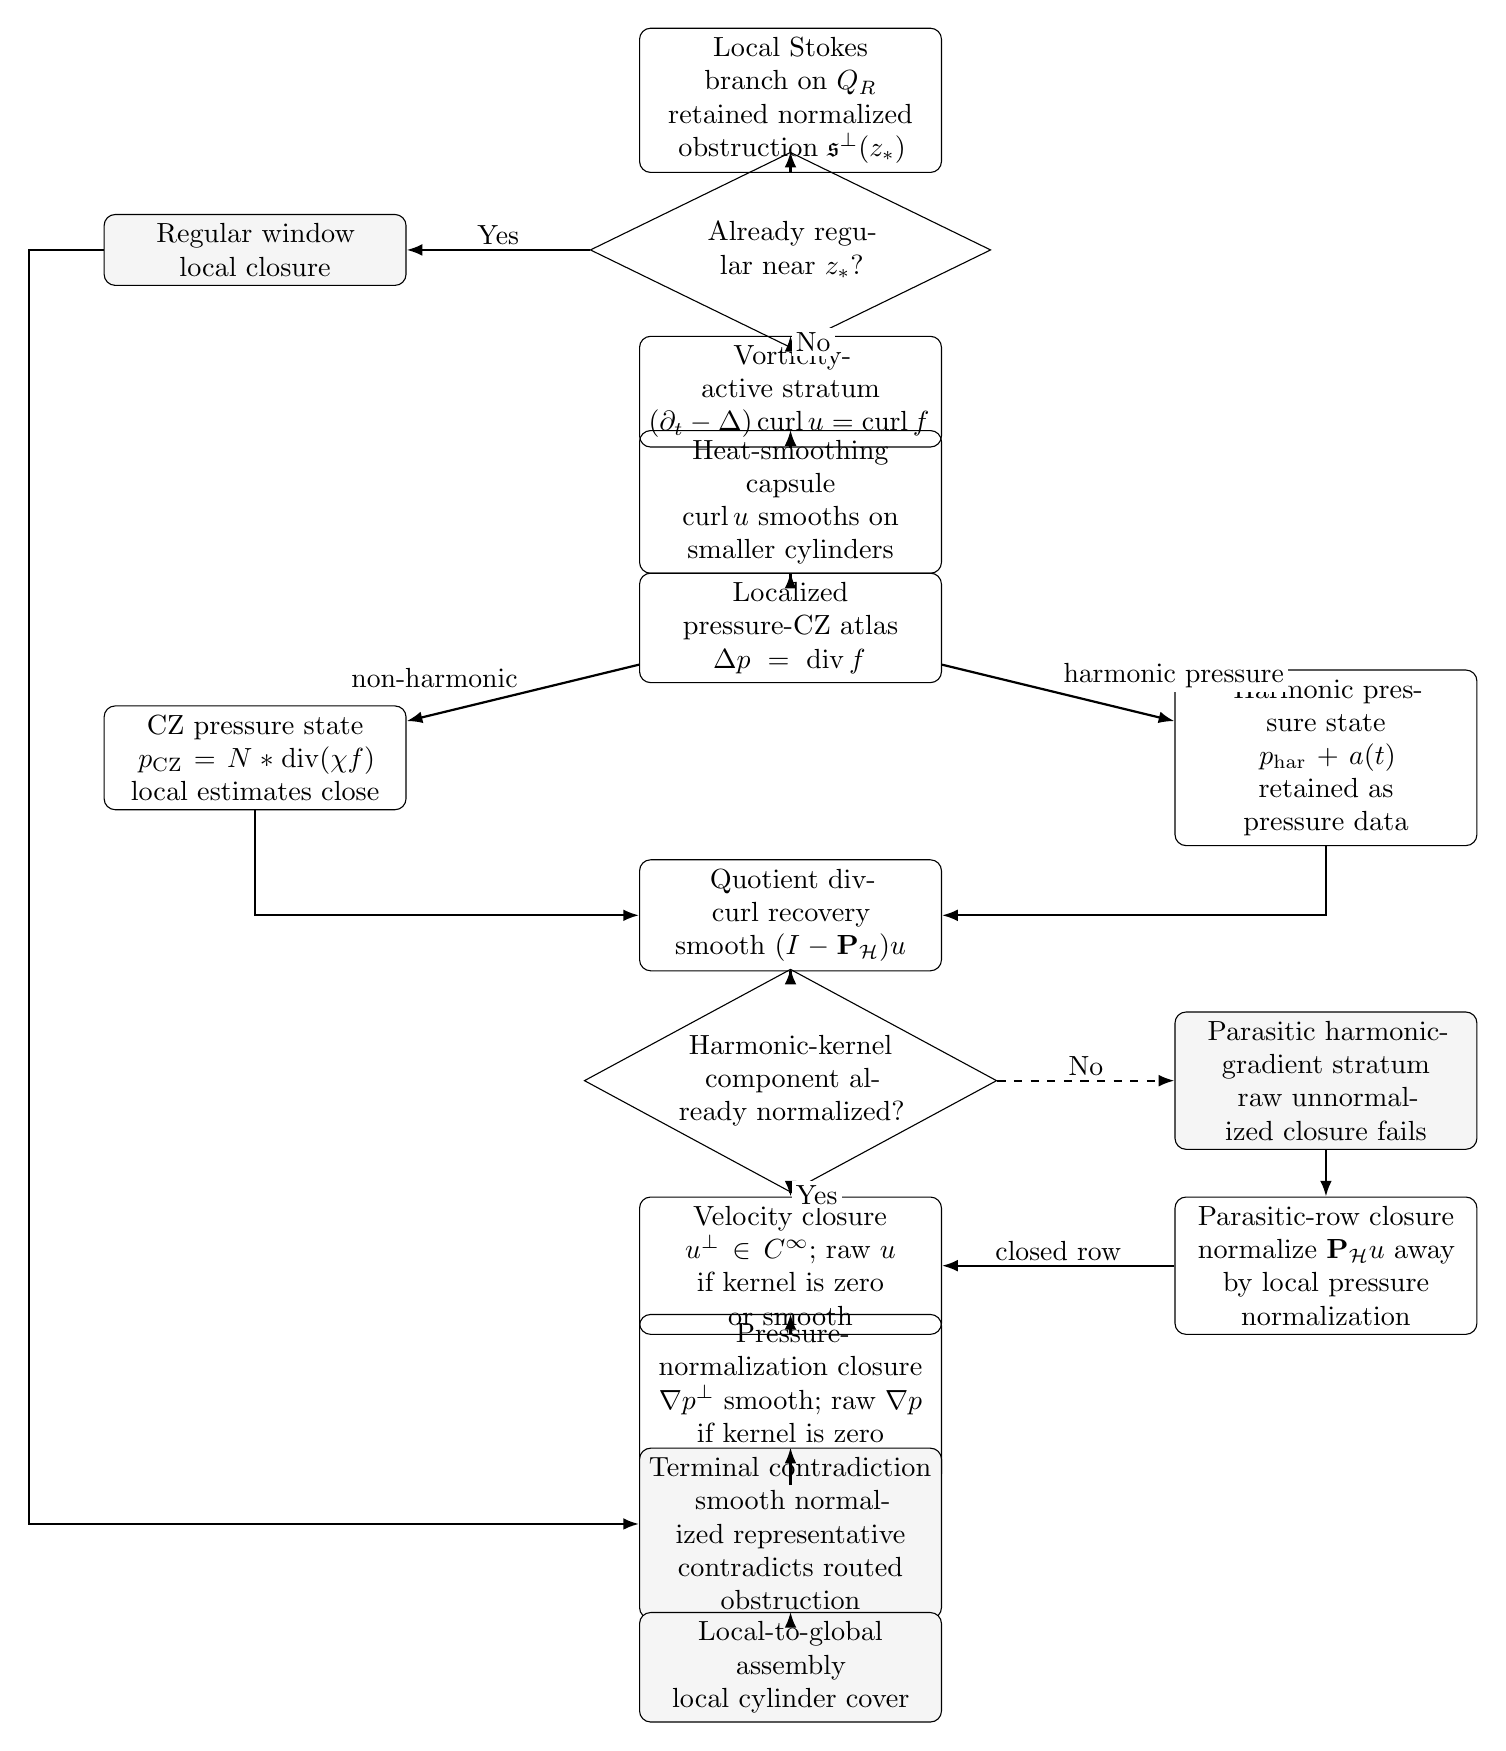
\begin{tikzpicture}[
  archnode/.style={draw, rounded corners, align=center, text width=36mm, minimum height=7mm},
  decision/.style={draw, diamond, aspect=2.05, align=center, text width=34mm, inner sep=1pt},
  terminal/.style={draw, rounded corners, align=center, text width=36mm, minimum height=7mm, fill=gray!8},
  arr/.style={-{Latex[length=2mm]}, thick},
  badarr/.style={-{Latex[length=2mm]}, thick, dashed},
  edgelabel/.style={fill=white, inner sep=1.5pt}
]
\node[archnode] (A) at (0,0.35) {Local Stokes branch on \(Q_R\)\\retained normalized obstruction \(\mathfrak s^\perp(z_*)\)};
\node[decision] (B) at (0,-1.55) {Already regular near \(z_*\)?};
\node[terminal] (REG) at (-6.8,-1.55) {Regular window\\local closure};
\node[archnode] (V) at (0,-3.35) {Vorticity-active stratum\\\((\partial_t-\Delta)\curl u=\curl f\)};
\node[archnode] (H) at (0,-4.75) {Heat-smoothing capsule\\\(\curl u\) smooths on smaller cylinders};
\node[archnode] (P) at (0,-6.35) {Localized pressure-CZ atlas\\\(\Delta p=\operatorname{div}f\)};
\node[archnode] (PCZ) at (-6.8,-8.0) {CZ pressure state\\\(p_{\mathrm{CZ}}=N*\operatorname{div}(\chi f)\)\\local estimates close};
\node[archnode] (PH) at (6.8,-8.0) {Harmonic pressure state\\\(p_{\mathrm{har}}+a(t)\)\\retained as pressure data};
\node[archnode] (D) at (0,-10.00) {Quotient div-curl recovery\\smooth \((I-\mathbf P_{\mathcal H})u\)};
\node[decision, text width=29mm, aspect=1.85] (K) at (0,-12.10) {Harmonic-kernel component already normalized?};
\node[terminal] (PAR) at (6.8,-12.10) {Parasitic harmonic-gradient stratum\\raw unnormalized closure fails};
\node[archnode] (PARC) at (6.8,-14.45) {Parasitic-row closure\\normalize \(\mathbf P_{\mathcal H}u\) away\\by local pressure normalization};
\node[archnode] (U) at (0,-14.45) {Velocity closure\\\(u^\perp\in C^\infty\); raw \(u\)\\if kernel is zero or smooth};
\node[archnode] (PG) at (0,-16.15) {Pressure-normalization closure\\\(\nabla p^\perp\) smooth; raw \(\nabla p\)\\if kernel is zero or smooth};
\node[terminal] (TC) at (0,-17.85) {Terminal contradiction\\smooth normalized representative\\contradicts routed obstruction};
\node[terminal] (G) at (0,-19.55) {Local-to-global assembly\\local cylinder cover};

\draw[arr] (A)--(B);
\draw[arr] (B)--node[edgelabel, above]{Yes}(REG);
\draw[arr] (B)--node[edgelabel, right]{No}(V);
\draw[arr] (V)--(H);
\draw[arr] (H)--(P);
\draw[arr] (P)--node[edgelabel, above left]{non-harmonic}(PCZ);
\draw[arr] (P)--node[edgelabel, above right]{harmonic pressure}(PH);
\draw[arr] (PCZ.south)--($(PCZ.south|-D.west)$)--(D.west);
\draw[arr] (PH.south)--($(PH.south|-D.east)$)--(D.east);
\draw[arr] (D)--(K);
\draw[badarr] (K)--node[edgelabel, above]{No}(PAR);
\draw[arr] (PAR)--(PARC);
\draw[arr] (PARC)--node[edgelabel, above]{closed row}(U);
\draw[arr] (K)--node[edgelabel, right]{Yes}(U);
\draw[arr] (U)--(PG);
\draw[arr] (PG)--(TC);
\draw[arr] (REG.west)--++(-0.95,0)|-($(TC.west)+(0,0.12)$);
\draw[arr] (TC)--(G);
\end{tikzpicture}
\end{adjustbox}
\caption{Stokes local proof graph produced by the construction algorithm.  The
analytic details are in \Cref{app:stokes-source}.  The dashed edge records the
raw parasitic harmonic-gradient failure; the solid descendant route closes
after local normalization.}
\label{fig:stokes-local-routing}
\end{figure}

\subsection{Architectural consequences}
The stress test isolates a concrete generated-PDE failure mode and shows how
Algorithm 1 handles it.  The vorticity route proves a quotient statement: it
controls the curl-determined component and leaves a harmonic-gradient residual.
The residual signature identifies the missing structure as representative
freedom in \(\calH(B_\rho)\), so the next local state is the
harmonic-kernel normalization state.  The invalid raw closure is thereby
converted into a normalized closure theorem plus an explicit compatibility
condition for raw representatives.

The example also shows the role of local PDE literature retrieval.  Once the
coordinate package is fixed, the required analytic inputs are standard local
estimates: heat smoothing, localized Calderon--Zygmund pressure decomposition,
quotient div-curl recovery, and harmonic-kernel normalization.  The
model-facing task is theorem matching inside that coordinate package: identify
the correct local theorem, state its hypotheses, apply it to the covered
component, and promote the residual term left outside its hypotheses.

The pressure and harmonic rows remain named states throughout the construction.
They enter through explicit local contracts rather than through an undeclared
whole-space projection, boundary condition, or global pressure convention.

\section{Lean Certificate for the Finite Proof State}
\label{sec:lean}

\subsection{Certification boundary}
\label{sec:certification-boundary}

The certified object is the construction ledger around the analytic estimates.
An estimate enters the graph as a named capsule with a declared local window,
input contract, output contract, pressure-representative or quotient status,
topology, retained obstruction, and failure route.  The certificate checks that
the capsule is invoked only after its input contract has been produced, that
its output is propagated with the declared topology and normalization, and that
each terminal closure consumes the obstruction assigned to its branch.  When a
reduction edge is present, the same ledger records that its target is already
closed or imported, its obstruction transport is declared, its analytic
coordinates are compatible with the target state, and its dependency is
acyclic.

Taxonomy completeness is also represented as a proof obligation.  Each local
state must declare its failure routes, and each terminal must declare its
status.  A regime discovered during audit is added as a new state, routed to an
existing closure by a valid reduction edge, or kept on the active frontier
until a closure, import, or reduction is supplied.  In a partial snapshot, such
a regime appears as an open obligation.  When an imported estimate is
corrected, strengthened, or rejected, branches outside its dependency cone keep
their status.

\subsection{Role of the backend}
The Lean backend is a finite certificate for the Stokes proof state.  The
capsule interfaces in \Cref{tab:stokes-capsules} are the manuscript-level
contracts; Lean represents their finite composition by a compressed state list,
transition relation, local closure inputs, terminal capsules, and imported
theorem boundaries.  The analytic Stokes estimates remain named imported
contracts.  The certificate checks the finite structure around those imports;
the PDE estimates themselves remain at the declared analytic boundary.

The checked Lean object mirrors the finite interface claims needed by the
Stokes stress test.  It contains fields for local-only assembly, finite state
coverage, manuscript display-name alignment, transition soundness, terminal
reachability, manuscript-label coverage, analytic-boundary coverage, pressure
localization, harmonic pressure bookkeeping, quotient continuity,
parasitic-row closure, and terminal capsule closure.

\subsection{Checked finite route structure}
The Lean certificate uses a compressed row list with eight states:
\[
\begin{gathered}
  \text{activity gate},\quad
  \text{vorticity heat},\quad
  \text{pressure-CZ normalization},\quad
  \text{quotient div-curl},\\
  \text{harmonic kernel},\quad
  \text{pressure normalization},\quad
  \text{empty residual state},\quad
  \text{terminal regularity}.
\end{gathered}
\]
The appendix and diagram display the finer analytic route states used for
exposition; this compressed Lean list groups those states into certificate rows.
The compression is the finite route abstraction checked by Lean; the analytic
proof remains the Stokes argument in \Cref{app:stokes-source}.
Lean checks that the row list is complete, duplicate-free, has length eight,
and carries the displayed manuscript names.  It also checks the transition
graph.  The transitions are ranked:
\[
  \rho(\text{activity gate})<\rho(\text{vorticity heat})<
  \cdots <\rho(\text{terminal regularity}),
\]
and every declared transition strictly increases this rank.  Thus the finite
route graph is acyclic.  Lean also proves that every listed state reaches
terminal regularity in the reflexive-transitive closure of the declared
transition relation.  The current Stokes stress test has no nontrivial
obstruction-reduction edges: its relevant branches close directly through local
capsules or through imported analytic contracts.  The general proof object
nonetheless records reduction edges as separate closure dependencies.

\subsection{Checked local assembly}
The global Stokes conclusion in the backend is pointwise by construction.  Its
input is a local closure assignment for every domain point.  Lean checks that
these local assignments assemble pointwise into the conclusion
\[
  \forall z\in\Omega,\ \exists K\ni z
  \quad u\text{ is smooth on }K
  \quad\text{and}\quad \nabla p\text{ is smooth on }K.
\]
This is the formal counterpart of the manuscript claim that global regularity
is assembled from local closures only.  The backend checks that the assembly
stage uses no global heat kernel, global projection, or exterior pressure
convention.

\subsection{Checked pressure and harmonic rows}
The pressure row is represented as a local atlas.  Lean checks that the
pressure-CZ source is localized before the CZ theorem is consumed, that the
local pressure decomposition carries a harmonic pressure remainder, and that
the harmonic remainder is retained as pressure-representative data.  The harmonic velocity row is
represented by a local projection state.  Lean checks that the projected
component is named, that the quotient carrier is available, and that the
normalization step records the removed harmonic component.

The backend also packages the parasitic-row closure.  The terminal capsule
consumes a harmonic-kernel closure input: either the kernel is smooth
or it has been normalized away.  This matches the mathematical stress test
above.

\subsection{Analytic boundary}
The Stokes backend treats the analytic estimates as named imported contracts.
The currently declared boundary is listed in
\Cref{tab:stokes-imported-contracts}.

\begingroup
\small
\begin{longtable}{@{}L{0.36\linewidth}L{0.54\linewidth}@{}}
\caption{Imported analytic contracts in the Stokes finite certificate.}
\label{tab:stokes-imported-contracts}\\
\toprule
Imported contract & Role in the finite proof state \\
\midrule
\endfirsthead
\caption[]{Imported analytic contracts in the Stokes finite certificate (continued).}\\
\toprule
Imported contract & Role in the finite proof state \\
\midrule
\endhead
Harmonic projection & Produces the local quotient and harmonic-kernel state. \\
\addlinespace
\(L^2\to H^{-1}\) curl bookkeeping & Places vorticity in the weak class needed
for heat smoothing. \\
\addlinespace
Smoothness of curled force & Supplies smooth forcing for the vorticity heat
equation. \\
\addlinespace
Local heat smoothing & Closes the vorticity regularity capsule. \\
\addlinespace
Local Calderon--Zygmund pressure & Produces the localized pressure atlas and
estimates for \(p_{\mathrm{CZ}}\). \\
\addlinespace
Pressure-representative gradient invariance & Records that pressure is compared only
modulo the allowed normalization. \\
\addlinespace
Local div-curl recovery & Recovers velocity from local curl and divergence data
modulo the harmonic kernel. \\
\addlinespace
Quotient div-curl recovery & Recovers the quotient representative
\((I-\mathbf P_{\mathcal H})u\). \\
\addlinespace
Time-parametrized quotient recovery & Supplies time-derivative estimates for
the quotient representative. \\
\bottomrule
\multicolumn{2}{@{}p{0.94\linewidth}@{}}{\footnotesize\emph{Note.}
Each row is an analytic import consumed by the finite proof-state certificate.  The
Lean layer checks where the import enters, which local state consumes it, and
which terminal claims depend on it.}\\
\end{longtable}
\endgroup

The axiom audit records the dependency boundary: the final validation
certificate depends on these named analytic imports, on the geometric compact
cylinder basis for open domains, and on standard Lean foundations.  The final
validation boundary lists these imports explicitly instead of introducing a
single final regularity axiom.

\subsection{Checked content}
Lean checks the finite repair structure: state coverage, absence of duplicate
states, strict transition ranking, terminal reachability, pointwise
local-to-global assembly, localization before pressure-CZ consumption, explicit
harmonic velocity and pressure-representative states, quotient continuity as a named
contract, harmonic pressure normalization as a named row, parasitic-row closure as
a terminal input, and exposure of the exact analytic boundary.  This layer
guards against global-estimate collapse.  A replacement of any imported
analytic estimate requires rechecking the capsules and dependency cones that
consume that estimate.

\section{Conclusion}
\label{sec:conclusion}

This paper proposes a construction method for PDE proofs and an AI-facing
architecture built around it.  The proof is built by the loop in
\Cref{alg:local-closure-residual-promotion}: choose an admissible local
coordinate package, match a theorem from the local PDE literature, close the
component covered by that theorem, promote the surviving remainder to a named
state, and choose the next normalization, quotient, topology, or decomposition
from the retained structure.  Standard PDE tools enter as local capsules rather
than as undeclared final shortcuts.  Reduction to a previously discharged
obstruction is represented by a separate acyclic closure dependency.  The
output is a finite, typed, auditable, and repairable analytic proof graph.

The Stokes stress test shows the construction in a closed linear setting.  The
local vorticity and pressure estimates close the non-harmonic contribution.
The remaining harmonic-gradient mode is promoted to a state, normalized by
quotient div-curl recovery and pressure compatibility, and closed as the
correct normalized theorem.  The raw representative is recovered only under the
zero-or-smooth compatibility condition.  The Lean backend checks the finite
certificate around this stress test and exposes the imported analytic boundary.
AI-assisted PDE proof development then proceeds through local analytic capsules
whose hypotheses, normalizations, compactness modes, obstructions, reduction
edges, and failure routes are recorded during construction, audit, and repair.
Each generated step must close a declared local component, import a named
theorem, reduce to a discharged obstruction, or expose the next residual state.

\appendix

\section{Implementation Capsule Template}
\label{app:implementation-capsule-template}

This appendix renders the implementation-phase capsule template as a
human-readable view of the canonical YAML certificate produced by the
construction step.  This phase proposes one local capsule, its theorem match,
its residual routes, and its outgoing obstruction transports.  It does not
perform the adversarial review.  The source is
\path{docs/source/strategy_papers/implementation_capsule_template.md}.

\VerbatimInput[fontsize=\small,frame=single]{implementation_capsule_template.md}

\section{Adversarial Evaluation Template}
\label{app:adversarial-evaluation-template}

This appendix renders the review-phase template.  The evaluator consumes an
implementation capsule and produces an independent adversarial report: schema
checks, theorem-match attacks, locality and representative attacks, residual
routing checks, obstruction-transport checks, and a final accept, revise, or
reject verdict.  The source is
\path{docs/source/strategy_papers/adversarial_evaluation_template.md}.

\VerbatimInput[fontsize=\small,frame=single]{adversarial_evaluation_template.md}

\section{Local Stokes Stress Test: Analytic Details}
\label{app:stokes-source}

\input{stokes_appendix_body.tex}

\begin{thebibliography}{99}

\bibitem{Necula97}
G. C. Necula.
Proof-carrying code.
\emph{Proceedings of the 24th ACM SIGPLAN-SIGACT Symposium on Principles of Programming Languages}, 106--119, 1997.

\bibitem{Lean15}
L. de Moura, S. Kong, J. Avigad, F. van Doorn, and J. von Raumer.
The Lean theorem prover.
\emph{Automated Deduction -- CADE-25}, Lecture Notes in Computer Science 9195, 378--388, 2015.

\bibitem{Lions1984a}
P.-L. Lions.
The concentration-compactness principle in the calculus of variations. The locally compact case, part 1.
\emph{Ann. Inst. H. Poincar\'e C Anal. Non Lin\'eaire} 1 (1984), no. 2, 109--145.

\bibitem{Lions1984b}
P.-L. Lions.
The concentration-compactness principle in the calculus of variations. The locally compact case, part 2.
\emph{Ann. Inst. H. Poincar\'e C Anal. Non Lin\'eaire} 1 (1984), no. 4, 223--283.

\bibitem{Gerard1998}
P. G\'erard.
Description du d\'efaut de compacit\'e de l'injection de Sobolev.
\emph{ESAIM Control Optim. Calc. Var.} 3 (1998), 213--233.

\bibitem{BahouriGerard1999}
H. Bahouri and P. G\'erard.
High frequency approximation of solutions to critical nonlinear wave equations.
\emph{Amer. J. Math.} 121 (1999), no. 1, 131--175.

\bibitem{Keraani2001}
S. Keraani.
On the defect of compactness for the Strichartz estimates of the Schr\"odinger equations.
\emph{J. Differential Equations} 175 (2001), no. 2, 353--392.

\bibitem{Stein1993}
E. M. Stein.
\emph{Harmonic Analysis: Real-Variable Methods, Orthogonality, and Oscillatory Integrals}.
Princeton Mathematical Series 43, Princeton University Press, 1993.

\bibitem{BahouriCheminDanchin2011}
H. Bahouri, J.-Y. Chemin, and R. Danchin.
\emph{Fourier Analysis and Nonlinear Partial Differential Equations}.
Grundlehren der mathematischen Wissenschaften 343, Springer, 2011.

\bibitem{CalderonZygmund1952}
A. P. Calder\'on and A. Zygmund.
On the existence of certain singular integrals.
\emph{Acta Math.} 88 (1952), 85--139.

\bibitem{Deniz2024}
E. Deniz.
Formalization of partial differential equations using HOL theorem proving.
Ph.D. thesis, Concordia University, 2024.

\bibitem{VanDoornMacbeth2024}
F. van Doorn and H. Macbeth.
Integrals within integrals: a formalization of the Gagliardo--Nirenberg--Sobolev inequality.
\emph{15th International Conference on Interactive Theorem Proving}, LIPIcs 309, 37:1--37:18, 2024.

\bibitem{Doll2025}
M. Doll.
Formalizing Schwartz functions and tempered distributions.
arXiv:2510.24060, 2025.

\bibitem{Gouezel2025}
S. Gou\"ezel.
Higher order differential calculus in mathlib.
arXiv:2509.04922, 2025.

\bibitem{ArmstrongKempe2026}
S. Armstrong and J. Kempe.
Formalization of De Giorgi--Nash--Moser theory in Lean.
arXiv:2604.05984, 2026.

\bibitem{LeanDojo2023}
K. Yang, A. M. Swope, A. Gu, R. Chalamala, P. Song, S. Yu, S. Godil, R. Prenger, and A. Anandkumar.
LeanDojo: theorem proving with retrieval-augmented language models.
\emph{Advances in Neural Information Processing Systems}, 2023.

\bibitem{LeanCopilot2024}
P. Song, K. Yang, and A. Anandkumar.
Lean Copilot: large language models as copilots for theorem proving in Lean.
arXiv:2404.12534, 2024.

\bibitem{CRAMF2025}
W. Lu, L. Du, S. Li, K. Weng, H. Sun, H. Liu, M. Yu, T. Zhang, and G. Yu.
Automated formalization via conceptual retrieval-augmented LLMs.
arXiv:2508.06931, 2025.

\bibitem{PDEController2025}
M. Soroco, J. Song, M. Xia, K. Emond, W. Sun, and W. Chen.
PDE-Controller: LLMs for autoformalization and reasoning of PDEs.
\emph{International Conference on Machine Learning}, 2025.

\bibitem{CodePDE2025}
S. Li, T. Marwah, J. Shen, W. Sun, A. Risteski, Y. Yang, and A. Talwalkar.
CodePDE: an inference framework for LLM-driven PDE solver generation.
arXiv:2505.08783, 2025.

\end{thebibliography}

\end{document}
